% Автоматаар үүсгэсэн — эх файл: lab05/README.md
\chapter{Лаб 5 — Өгөгдлийн шугам ба холбоос тасрах}

\begingroup\scriptsize\begin{longtable}[]{@{}ll@{}}
\toprule
\endhead
\textbf{7 хоног} & XI\tabularnewline
\textbf{Хугацаа} & 4 цаг\tabularnewline
\textbf{Суралцахуйн үр дүн} & ҮД4 (үнэлэх), ҮД6, ҮД7\tabularnewline
\textbf{Үнэлгээ} & Бичгийн тайлан, 10 оноо\tabularnewline
\textbf{Гол хэмжилт} & Store-and-forward-ийн алдагдал, \textbf{RPO} ба \textbf{MTTR} секундээр\tabularnewline
\bottomrule
\end{longtable}\endgroup

\hypertarget{ux437ux43eux440ux438ux43bux433ux43e}{%
\section{1. Зорилго}\label{ux437ux43eux440ux438ux43bux433ux43e}}

Хоёр хагас. Эхний хагаст {[}ЗК{]} үүл дээр бүрэн өгөгдлийн шугам барина:

\begin{verbatim}
[Pi] mosquitto ══гүүр══▶ [ЗК] EMQX ─▶ Node-RED ─▶ InfluxDB 3 ─▶ Grafana
                                   (задлах,     (хадгалах)    (харах)
                                    шалгах)  └─▶ dead-letter
\end{verbatim}

Хоёр дахь хагас --- \textbf{энэ бол лабораторийн зүрх} --- өгсөх урсгалыг (uplink) тасалж, юу амьд үлдэхийг тоогоор хэмжинэ. Хоёр тоог гаргана:

\begin{itemize}
\tightlist
\item
  \textbf{RPO} (Recovery Point Objective) --- хэдэн секундын өгөгдөл \textbf{бүрмөсөн алдагдав}
\item
  \textbf{MTTR} (Mean Time To Recovery) --- шугам бүрэн эдгэрэх хүртэл хэдэн секунд өнгөрөв
\end{itemize}

\begin{quote}
\textbf{Курсын тодорхойлолт.} RPO нь угтаа "хэдий хэмжээний өгөгдлийн алдагдлыг (хугацаагаар) хүлээн зөвшөөрөх вэ" гэсэн \textbf{зорилт}; MTTR нь олон эвдрэлийн сэргэх хугацааны \textbf{дундаж}. Энэ лабораторид бид нэг туршилт бүрийн \textbf{бодит} утгыг хэмжинэ: RPO = бүрмөсөн алдагдсан хамгийн урт тасралтгүй хэсгийн үргэлжлэл (с); MTTR = өгсөх урсгал сэргэснээс хойш тасалдлын үеэр илгээсэн сүүлийн мессеж санд хүрэх хүртэлх хугацаа (с). Олон давталтын дундаж нь жинхэнэ MTTR болно.
\end{quote}

Энэ хоёр өөр үзүүлэлт: систем 5 секундын дараа сэргэж болно (сайн MTTR), гэхдээ тэр хугацааны өгөгдөл бүрэн алдагдсан байж болно (муу RPO).

\begin{quote}
\textbf{⚠ ЭНЭ ЛАБОРАТОРИЙН ХАМГИЙН ЧУХАЛ УРХИ.} Өгсөх урсгал сэргэхэд гүүр хуримтлагдсан мессежээ \textbf{нэг тэсрэлтээр} урсгана. Хэрэв та \texttt{mosquitto\_sub}-ыг тэр тэсрэлтийн \textbf{дараа} асаавал юу ч харагдахгүй --- MQTT нь өнгөрсөн мессежийг шинэ захиалагчид дахин илгээхгүй. Тэгээд "store-and-forward ажиллаагүй" гэсэн \textbf{буруу дүгнэлт} гарна. Дахин илгээлт болсон эсэхийг \textbf{зөвхөн InfluxDB дотор} (эсвэл эхнээс нь ажиллаж байсан тогтвортой session-тэй захиалагчаар) шалгана.
\end{quote}

\hypertarget{ux443ux440ux44cux434ux447ux438ux43bux441ux430ux43d-ux43dux4e9ux445ux446ux4e9ux43b}{%
\section{2. Урьдчилсан нөхцөл}\label{ux443ux440ux44cux434ux447ux438ux43bux441ux430ux43d-ux43dux4e9ux445ux446ux4e9ux43b}}

\begin{itemize}
\tightlist
\item
  Лаб 1--4 дууссан, \texttt{lab04-done} тэмдэглэгээ тавигдсан
\item
  {[}ЗК{]} \texttt{pipeline} профайл нэмж асаана:
\end{itemize}

\begin{Shaded}
\begin{Highlighting}[]
\BuiltInTok{cd}\NormalTok{ \textasciitilde{}/cnc302/stack }\KeywordTok{\&\&} \FunctionTok{make}\NormalTok{ up{-}pipeline }\KeywordTok{\&\&} \FunctionTok{make}\NormalTok{ health}
\ExtensionTok{docker}\NormalTok{ compose ps       \# nodered }\StringTok{"healthy"}\NormalTok{ болтол 40 сек хүлээнэ}
\end{Highlighting}
\end{Shaded}

\begin{itemize}
\tightlist
\item
  {[}Pi{]} Pi дээр \texttt{sudo} эрх (\texttt{uplink-down} нь iptables/nft, \texttt{disk} нь mount шаарддаг)
\item
  {[}Pi{]} \texttt{stress-ng} суусан: \texttt{sudo\ apt\ install\ -y\ stress-ng}
\item
  {[}Pi{]} Гүүр ажиллаж байна: \texttt{cd\ \textasciitilde{}/cnc302/edge\ \&\&\ make\ link} → \texttt{bridge/state\ 1}
\item
  {[}Pi{]} Терминал бүрд: \texttt{set\ -a\ \&\&\ source\ \textasciitilde{}/cnc302/edge/.env\ \&\&\ set\ +a}
\end{itemize}

\hypertarget{ux43eux43dux43eux43bux44bux43d-ux441ux430ux43dux443ux443ux43bux433ux430}{%
\section{3. Онолын сануулга}\label{ux43eux43dux43eux43bux44bux43d-ux441ux430ux43dux443ux443ux43bux433ux430}}

\hypertarget{ux431ux430ux442ux430ux43bux433ux430ux430-ux43dux44c-ux434ux430ux432ux445ux430ux440ux433ux443ux443ux434ux44bux43d-ux4afux440ux436ux432ux44dux440-ux431ux438ux448-ux445ux430ux43cux433ux438ux439ux43d-ux441ux443ux43b-ux445ux43eux43bux431ux43eux43eux441ux43eux43eux440-ux442ux43eux434ux43eux440ux445ux43eux439ux43bux43eux433ux434ux43eux43dux43e}{%
\subsection{Баталгаа нь давхаргуудын үржвэр биш, хамгийн сул холбоосоор тодорхойлогдоно}\label{ux431ux430ux442ux430ux43bux433ux430ux430-ux43dux44c-ux434ux430ux432ux445ux430ux440ux433ux443ux443ux434ux44bux43d-ux4afux440ux436ux432ux44dux440-ux431ux438ux448-ux445ux430ux43cux433ux438ux439ux43d-ux441ux443ux43b-ux445ux43eux43bux431ux43eux43eux441ux43eux43eux440-ux442ux43eux434ux43eux440ux445ux43eux439ux43bux43eux433ux434ux43eux43dux43e}}

QoS 2-оор илгээсэн мессеж брокерт баттай хүрнэ. Гэвч брокероос Node-RED, тэндээс InfluxDB руу явах замд MQTT-ийн баталгаа \textbf{байхгүй}. Тиймээс "төгсгөл-төгсгөлийн найдвартай байдал" гэдэг нь давхарга бүрийн баталгааны нийлбэр биш --- \textbf{хамгийн сул холбоос} юм.

\hypertarget{ux445ux430ux430ux43dux430-ux431ux443ux444ux435ux440ux43bux44dux433ux434ux44dux445-ux432ux44d}{%
\subsection{Хаана буферлэгдэх вэ}\label{ux445ux430ux430ux43dux430-ux431ux443ux444ux435ux440ux43bux44dux433ux434ux44dux445-ux432ux44d}}

\begingroup\scriptsize\begin{longtable}[]{@{}lll@{}}
\toprule
\begin{minipage}[b]{0.30\columnwidth}\raggedright
Эвдрэл\strut
\end{minipage} & \begin{minipage}[b]{0.30\columnwidth}\raggedright
Хэн буферлэдэг\strut
\end{minipage} & \begin{minipage}[b]{0.30\columnwidth}\raggedright
Хязгаар\strut
\end{minipage}\tabularnewline
\midrule
\endhead
\begin{minipage}[t]{0.30\columnwidth}\raggedright
\textbf{Өгсөх урсгал тасарсан}\strut
\end{minipage} & \begin{minipage}[t]{0.30\columnwidth}\raggedright
ирмэгийн mosquitto-гийн гүүрний дараалал (\textbf{RAM}, үе үе microSD руу хуулна)\strut
\end{minipage} & \begin{minipage}[t]{0.30\columnwidth}\raggedright
\texttt{max\_\allowbreak{}queued\_\allowbreak{}messages} / \texttt{max\_\allowbreak{}queued\_\allowbreak{}bytes}, контейнерийн RAM (128 MiB)\strut
\end{minipage}\tabularnewline
\begin{minipage}[t]{0.30\columnwidth}\raggedright
Ирмэгийн брокер унтарсан\strut
\end{minipage} & \begin{minipage}[t]{0.30\columnwidth}\raggedright
төхөөрөмж өөрөө (кодлогдсон бол)\strut
\end{minipage} & \begin{minipage}[t]{0.30\columnwidth}\raggedright
төхөөрөмжийн RAM\strut
\end{minipage}\tabularnewline
\begin{minipage}[t]{0.30\columnwidth}\raggedright
Node-RED/InfluxDB унтарсан\strut
\end{minipage} & \begin{minipage}[t]{0.30\columnwidth}\raggedright
Node-RED-ийн dead-letter файл\strut
\end{minipage} & \begin{minipage}[t]{0.30\columnwidth}\raggedright
диск\strut
\end{minipage}\tabularnewline
\begin{minipage}[t]{0.30\columnwidth}\raggedright
Диск дүүрсэн\strut
\end{minipage} & \begin{minipage}[t]{0.30\columnwidth}\raggedright
\textbf{хэн ч үгүй}\strut
\end{minipage} & \begin{minipage}[t]{0.30\columnwidth}\raggedright
---\strut
\end{minipage}\tabularnewline
\bottomrule
\end{longtable}\endgroup

\hypertarget{store-and-forward-ux438ux439ux43d-ux433ux443ux440ux432ux430ux43d-ux442ux43eux445ux438ux440ux433ux43eux43e}{%
\subsection{Store-and-forward-ийн гурван тохиргоо}\label{store-and-forward-ux438ux439ux43d-ux433ux443ux440ux432ux430ux43d-ux442ux43eux445ux438ux440ux433ux43eux43e}}

\texttt{edge/\allowbreak{}mosquitto/\allowbreak{}mosquitto.\allowbreak{}conf} ба \texttt{conf.\allowbreak{}d/\allowbreak{}bridge.\allowbreak{}conf} дахь гурван мөр л энэ бүхнийг тодорхойлно:

\begingroup\scriptsize\begin{longtable}[]{@{}lll@{}}
\toprule
\begin{minipage}[b]{0.30\columnwidth}\raggedright
Тохиргоо\strut
\end{minipage} & \begin{minipage}[b]{0.30\columnwidth}\raggedright
Хаана\strut
\end{minipage} & \begin{minipage}[b]{0.30\columnwidth}\raggedright
Үүрэг\strut
\end{minipage}\tabularnewline
\midrule
\endhead
\begin{minipage}[t]{0.30\columnwidth}\raggedright
\texttt{cleansession\ false}\strut
\end{minipage} & \begin{minipage}[t]{0.30\columnwidth}\raggedright
bridge.conf\strut
\end{minipage} & \begin{minipage}[t]{0.30\columnwidth}\raggedright
тасрахад \textbf{алсын} (EMQX) талын захиалга, session хадгалагдана; \texttt{true} бол холбоос тасрахад алсын захиалга, мессеж цэвэрлэгдэнэ\strut
\end{minipage}\tabularnewline
\begin{minipage}[t]{0.30\columnwidth}\raggedright
\texttt{local\_\allowbreak{}cleansession\ false}\strut
\end{minipage} & \begin{minipage}[t]{0.30\columnwidth}\raggedright
bridge.conf\strut
\end{minipage} & \begin{minipage}[t]{0.30\columnwidth}\raggedright
гүүрний \textbf{локал} талын session (гүүрт зориулсан дараалал) хадгалагдана. Заагаагүй бол \texttt{cleansession}-ий утгыг авна\strut
\end{minipage}\tabularnewline
\begin{minipage}[t]{0.30\columnwidth}\raggedright
\texttt{queue\_\allowbreak{}qos0\_\allowbreak{}messages\ true}\strut
\end{minipage} & \begin{minipage}[t]{0.30\columnwidth}\raggedright
mosquitto.conf (\textbf{глобал})\strut
\end{minipage} & \begin{minipage}[t]{0.30\columnwidth}\raggedright
тогтвортой клиент (гүүр) тасарсан үед QoS 0 мессежийг ч дараалалд оруулна (MQTT стандарт биш сонголт); эдгээр нь \texttt{max\_\allowbreak{}queued\_\allowbreak{}messages}-д тоологдоно\strut
\end{minipage}\tabularnewline
\bottomrule
\end{longtable}\endgroup

\begin{figure}
\centering
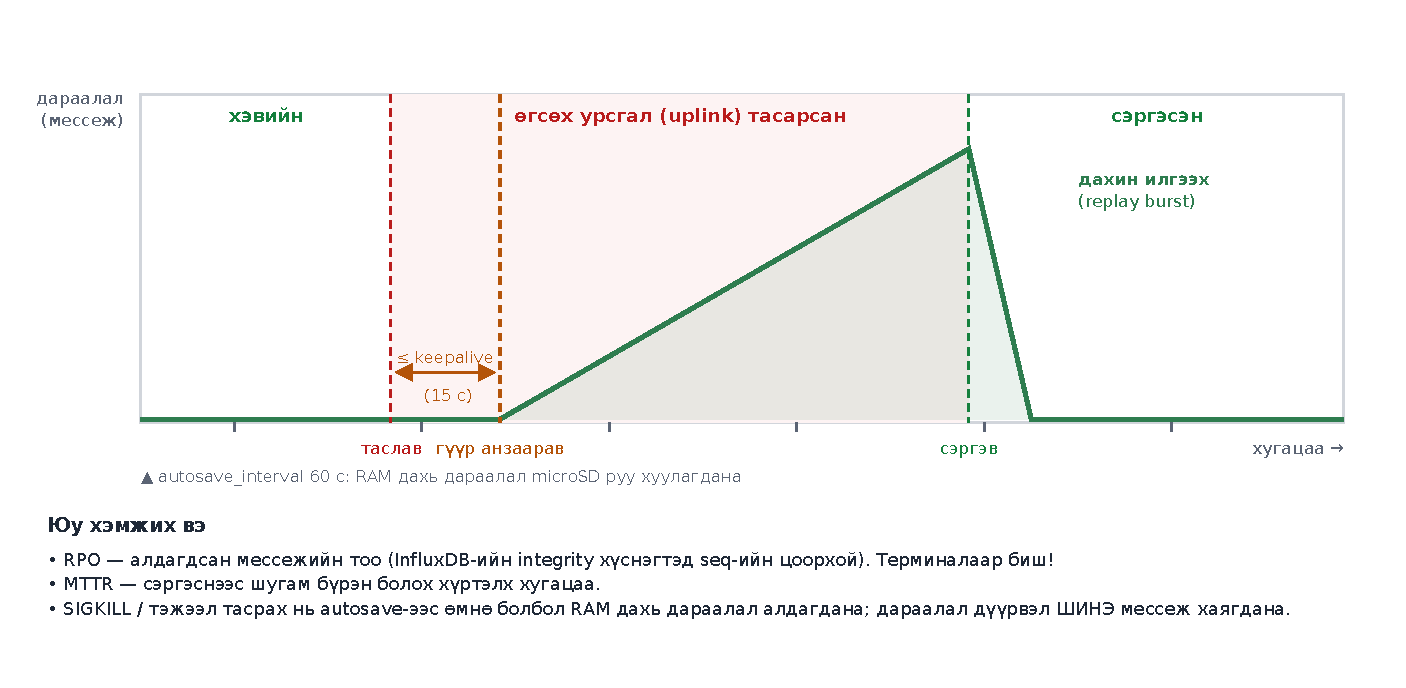
\includegraphics{figures/fig-bridge-saf.pdf}
\caption{Зураг 5.2 --- Store-and-forward: холбоос тасрахад ирмэгийн Mosquitto мессежийг дараалалд хадгалж, сэргэхэд дахин илгээнэ}
\end{figure}

\begin{quote}
\textbf{⚠ Тохиргооны урхи:} \texttt{bridge\_\allowbreak{}queue\_\allowbreak{}qos0\_\allowbreak{}messages} гэсэн сонголт \textbf{байхгүй} --- mosquitto үүнийг танихгүй сонголт гэж үзээд \textbf{огт эхлэхгүй}. Зөв нэр нь глобал \texttt{queue\_\allowbreak{}qos0\_\allowbreak{}messages}. Гүүрний хэсэгт бичих гэж оролдвол \texttt{docker\ compose\ logs\ mosquitto} дотор \texttt{Unknown\ configuration\ variable} гарна.
\end{quote}

\textbf{Хүлээгдэх зан төлөв:} эдгээр гурав зөв тохируулагдсан үед \textbf{QoS 1}-ээр өгсөх урсгал унасан хугацаанд нийтэлсэн мессеж бүгд дараалалд орж, холбоос сэргэхэд үүл рүү урсана. Гэхдээ дөрвөн нарийн зүйл RPO/MTTR-ын тоонд шууд нөлөөлнө:

\begin{enumerate}
\def\labelenumi{\arabic{enumi}.}
\tightlist
\item
  \textbf{Гүүр тасралтыг шууд мэддэггүй.} iptables DROP нь TCP холболтыг "тасалдаггүй" --- пакетууд зүгээр л алга болно. Гүүр \texttt{keepalive\_\allowbreak{}interval} (анхдагч \textbf{60 с}) хугацаанд юу ч ирээгүй бол PING илгээж, хариу ирэхгүй бол холболтыг хаана. Тэр болтол \texttt{bridge/state} = 1 хэвээр. Иймээс \textbf{60 секундын тасалдалд \texttt{bridge.jsonl} дээр "0" огт гарахгүй байж болно} (бидний туршилтаар keepalive 60 үед 60 с тасалдалд "0" гараагүй, keepalive 10 үед \textasciitilde19 с-т илэрсэн). Тиймээс энэ лабд тасалдлын \textbf{бодит} цагийг \texttt{failure\_\allowbreak{}inject.\allowbreak{}sh} бичдэг \texttt{uplink-events.\allowbreak{}jsonl}-ээс авна (\texttt{verify\ -\/\allowbreak{}-cut-log}).
\item
  \textbf{QoS 0 ба илрүүлэх хугацаа.} Гүүр тасралтыг илрүүлэхээс өмнө TCP холболт руу бичигдсэн QoS 0 мессежийг дахин илгээх механизм байхгүй (QoS 0 = "хамгийн ихдээ нэг удаа"). Тиймээс \texttt{queue\_\allowbreak{}qos0\_\allowbreak{}messages\ true} байсан ч QoS 0-ийн алдагдал ≈ \emph{хурд × илрүүлэх хугацаа} байж болно. QoS 1 мессеж PUBACK авах хүртэл session-д үлдэж, дахин холбогдоход дахин илгээгдэнэ.
\item
  \textbf{Дараалал дүүрэхэд ШИНЭ мессеж хаягдана.} Албан ёсны баримтаар хязгаарт хүрсний дараах мессежүүд "чимээгүй хаягдана" --- хуучин нь үлдэнэ. mosquitto лог дээр \texttt{Outgoing\ messages\ are\ being\ dropped\ for\ client\ local.\allowbreak{}edge-\ldots{}} гарна.
\item
  \textbf{Дараалал RAM-д байна.} \texttt{persistence\ true} үед санах ой дахь өгөгдөл \texttt{mosquitto.db} файлд зөвхөн (а) \texttt{autosave\_\allowbreak{}interval} тутамд, (б) mosquitto \textbf{хэвийн} унтрахад, (в) \texttt{SIGUSR1} дохиогоор бичигдэнэ. \texttt{autosave\_\allowbreak{}on\_\allowbreak{}changes\ false} тул манай тохиргоонд 60 секунд тутамд. \textbf{Цахилгаан гэнэт тасарвал} (эсвэл SIGKILL) сүүлийн хадгалалтаас хойш дараалалд орсон мессеж алдагдана --- энэ нь RPO-д шууд нэмэгдэнэ.
\end{enumerate}

Гүүр тасарснаа мэдсэний дараа \texttt{restart\_\allowbreak{}timeout\ 5\ 60}-ийн дагуу 5 секундээс эхлэн 60 секунд хүртэл санамсаргүй өсөх ("Decorrelated Jitter") завсарлагатайгаар дахин холбогдохыг оролдоно --- энэ нь MTTR-д нэмэгдэнэ.

\begin{quote}
Албан ёсны баримт: \href{https://mosquitto.org/man/mosquitto-conf-5.html}{mosquitto.conf(5)} --- \texttt{max\_\allowbreak{}queued\_\allowbreak{}messages}, \texttt{max\_\allowbreak{}queued\_\allowbreak{}bytes}, \texttt{queue\_\allowbreak{}qos0\_\allowbreak{}messages}, \texttt{persistence}, \texttt{autosave\_\allowbreak{}interval}, \texttt{cleansession}, \texttt{local\_\allowbreak{}cleansession}, \texttt{keepalive\_\allowbreak{}interval}, \texttt{restart\_timeout}.
\end{quote}

\hypertarget{ux430ux43bux445ux43cux443ux443ux434}{%
\section{4. Алхмууд}\label{ux430ux43bux445ux43cux443ux443ux434}}

\hypertarget{ux430ux43bux445ux430ux43c-1-influxdb-ux431ux44dux43bux442ux433ux44dux445-ux431ux430-ux431ux438ux447ux438ux43bux442ux438ux439ux433-ux433ux430ux440ux430ux430ux440-ux448ux430ux43bux433ux430ux445-25-ux43cux438ux43d-ux437ux43a}{%
\subsection{Алхам 1 --- InfluxDB бэлтгэх ба бичилтийг гараар шалгах (25 мин) {[}ЗК{]}}\label{ux430ux43bux445ux430ux43c-1-influxdb-ux431ux44dux43bux442ux433ux44dux445-ux431ux430-ux431ux438ux447ux438ux43bux442ux438ux439ux433-ux433ux430ux440ux430ux430ux440-ux448ux430ux43bux433ux430ux445-25-ux43cux438ux43d-ux437ux43a}}

InfluxDB 3 нь \emph{schema-on-write}: анхны бичилт өгөгдлийн сан, хүснэгтийг автоматаар үүсгэдэг. Гэхдээ санг \textbf{ил үүсгэх} нь сайн дадал (нэр, хадгалах хугацааг өөрөө шийднэ). Амжилттай бол \texttt{200}, аль хэдийн байвал \texttt{409} буцна.

\begin{Shaded}
\begin{Highlighting}[]
\ExtensionTok{curl}\NormalTok{ {-}s {-}w }\StringTok{\textquotesingle{}  → HTTP \%\{http\_code\}\textbackslash{}n\textquotesingle{}}\NormalTok{ {-}X POST }\StringTok{\textquotesingle{}http://localhost:8181/api/v3/configure/database\textquotesingle{}} \KeywordTok{\textbackslash{}}
  \ExtensionTok{{-}H} \StringTok{\textquotesingle{}Content{-}Type: application/json\textquotesingle{}}\NormalTok{ {-}d }\StringTok{\textquotesingle{}\{"db":"cnc302"\}\textquotesingle{}}
\ExtensionTok{curl}\NormalTok{ {-}s }\StringTok{\textquotesingle{}http://localhost:8181/api/v3/configure/database?format=json\textquotesingle{}} \KeywordTok{|} \ExtensionTok{jq}
\CommentTok{\# Нэг мөр гараар бичиж, буцааж уншина}
\ExtensionTok{curl}\NormalTok{ {-}s {-}X POST }\StringTok{\textquotesingle{}http://localhost:8181/api/v3/write\_lp?db=cnc302\&precision=millisecond\textquotesingle{}} \KeywordTok{\textbackslash{}}
  \ExtensionTok{{-}H} \StringTok{\textquotesingle{}Content{-}Type: text/plain\textquotesingle{}} \KeywordTok{\textbackslash{}}
  \ExtensionTok{{-}{-}data{-}binary} \StringTok{"telemetry,site=test,device=test0 temperature=24.5 }\VariableTok{$(}\FunctionTok{date}\NormalTok{ +\%s\%3N}\VariableTok{)}\StringTok{"}

\ExtensionTok{curl}\NormalTok{ {-}s {-}X POST }\StringTok{\textquotesingle{}http://localhost:8181/api/v3/query\_sql\textquotesingle{}} \KeywordTok{\textbackslash{}}
  \ExtensionTok{{-}H} \StringTok{\textquotesingle{}Content{-}Type: application/json\textquotesingle{}} \KeywordTok{\textbackslash{}}
  \ExtensionTok{{-}d} \StringTok{\textquotesingle{}\{"db":"cnc302","q":"SELECT * FROM telemetry LIMIT 5","format":"json"\}\textquotesingle{}} \KeywordTok{|} \ExtensionTok{jq}
\CommentTok{\# Ижил асуулга GET{-}ээр (URL{-}кодчилсон), мөр бүр тусдаа JSON (jsonl):}
\ExtensionTok{curl}\NormalTok{ {-}s }\StringTok{\textquotesingle{}http://localhost:8181/api/v3/query\_sql?db=cnc302\&format=jsonl\&q=SELECT+*+FROM+telemetry+LIMIT+5\textquotesingle{}}
\end{Highlighting}
\end{Shaded}

\begin{itemize}
\tightlist
\item
  \texttt{precision} утга нь v3 API-д \textbf{бүтэн үгээр}: \texttt{auto} (анхдагч) \textbar{} \texttt{nanosecond} \textbar{} \texttt{microsecond} \textbar{} \texttt{millisecond} \textbar{} \texttt{second}. \texttt{ms}, \texttt{s} гэх товчлол нь зөвхөн v1 (\texttt{/write}) ба v2 (\texttt{/api/v2/write}) нийцлийн API-д хүчинтэй.
\item
  Амжилттай бичилт \texttt{204\ No\ Content} буцаана. Line protocol буруу эсвэл баганын төрөл зөрчигдвөл \texttt{400} ба алдааны JSON (анхдагч \texttt{accept\_\allowbreak{}partial=\allowbreak{}true} үед зөв мөрүүд нь бичигдэнэ).
\item
  \texttt{query\_sql}-ийн \texttt{format}: \texttt{json} (анхдагч), \texttt{jsonl}, \texttt{csv}, \texttt{pretty}, \texttt{parquet}.
\item
  \textbf{Нэвтрэлт:} манай стек \texttt{-\/-without-auth}-аар ажилладаг (\textbf{зөвхөн лабораторид}). Бодит системд эхлээд \texttt{docker\ exec\ -it\ cnc302-influxdb\ influxdb3\ create\ token\ -\/\allowbreak{}-admin} гэж токен үүсгэж, бүх хүсэлтэд \texttt{-H\ "Authorization:\allowbreak{}\ Bearer\ \$TOKEN"} толгой нэмнэ (\texttt{data\_\allowbreak{}integrity.\allowbreak{}py\ verify\ -\/\allowbreak{}-auth-token\ \ldots{}}).
\end{itemize}

\begin{quote}
Албан ёсны баримт: \href{https://docs.influxdata.com/influxdb3/core/write-data/http-api/v3-write-lp/}{InfluxDB 3 Core --- v3 write\_\allowbreak{}lp API}, \href{https://docs.influxdata.com/influxdb3/core/query-data/execute-queries/influxdb-v3-api/}{v3 query API}
\end{quote}

\textbf{Бичилтийн саатлыг хэмжинэ} (5 удаа давтаж, \texttt{\%\{time\_total\}}-ыг тэмдэглэ):

\begin{Shaded}
\begin{Highlighting}[]
\KeywordTok{for} \ExtensionTok{i}\NormalTok{ in 1 2 3 4 5}\KeywordTok{;} \KeywordTok{do} \ExtensionTok{curl}\NormalTok{ {-}s {-}o /dev/null {-}w }\StringTok{\textquotesingle{}\%\{time\_total\}\textbackslash{}n\textquotesingle{}}\NormalTok{ {-}X POST }\KeywordTok{\textbackslash{}}
  \StringTok{\textquotesingle{}http://localhost:8181/api/v3/write\_lp?db=cnc302\&precision=millisecond\textquotesingle{}} \KeywordTok{\textbackslash{}}
  \ExtensionTok{{-}H} \StringTok{\textquotesingle{}Content{-}Type: text/plain\textquotesingle{}} \KeywordTok{\textbackslash{}}
  \ExtensionTok{{-}{-}data{-}binary} \StringTok{"telemetry,site=test,device=test0 temperature=2}\VariableTok{$i}\StringTok{.0 }\VariableTok{$(}\FunctionTok{date}\NormalTok{ +\%s\%3N}\VariableTok{)}\StringTok{"}\KeywordTok{;} \KeywordTok{done}
\end{Highlighting}
\end{Shaded}

\hypertarget{ux445ux4afux441ux43dux44dux433ux442-5.1-ux431ux438ux447ux438ux445-ux434ux430ux432ux445ux430ux440ux433ux44bux43d-ux441ux443ux443ux440ux44c}{%
\subsubsection{Хүснэгт 5.1 --- Бичих давхаргын суурь}\label{ux445ux4afux441ux43dux44dux433ux442-5.1-ux431ux438ux447ux438ux445-ux434ux430ux432ux445ux430ux440ux433ux44bux43d-ux441ux443ux443ux440ux44c}}

\begingroup\scriptsize\begin{longtable}[]{@{}lll@{}}
\toprule
Хэмжигдэхүүн & Утга & Тэмдэглэл\tabularnewline
\midrule
\endhead
\texttt{write\_lp} дундаж хугацаа (мс) & & 5 хэмжилтийн дундаж\tabularnewline
\texttt{write\_lp} хамгийн удаан (мс) & &\tabularnewline
Хариу код (амжилттай бичилт) & & 204 хүлээгдэнэ\tabularnewline
\texttt{query\_sql} мөр буцаав уу & &\tabularnewline
\bottomrule
\end{longtable}\endgroup

\begin{quote}
InfluxDB 2.7 нөөц хувилбар дээр ажиллаж байгаа бол \texttt{docs/\allowbreak{}troubleshooting.\allowbreak{}md} §6-г уншаад цаашид \texttt{verify}-д \texttt{-\/-influx2} тугийг нэмнэ.
\end{quote}

\hypertarget{ux430ux43bux445ux430ux43c-2-node-red-ux448ux443ux433ux430ux43c-ux431ux430-grafana-ux441ux430ux43cux431ux430ux440-45-ux43cux438ux43d-ux437ux43a}{%
\subsection{Алхам 2 --- Node-RED шугам ба Grafana самбар (45 мин) {[}ЗК{]}}\label{ux430ux43bux445ux430ux43c-2-node-red-ux448ux443ux433ux430ux43c-ux431ux430-grafana-ux441ux430ux43cux431ux430ux440-45-ux43cux438ux43d-ux437ux43a}}

\textbf{2.1 Импортлох.} Node-RED (\texttt{:1880}) → ☰ → \textbf{Import} (эсвэл \texttt{Ctrl-I}) → \texttt{lab05/\allowbreak{}flows/\allowbreak{}nodered-pipeline.\allowbreak{}json}-ийн агуулгыг наах эсвэл файлыг сонгох → \textbf{new flow} → \textbf{Import} → \textbf{Deploy}.

\begin{quote}
Албан ёсны баримт: \href{https://nodered.org/docs/user-guide/editor/workspace/import-export}{Node-RED --- Importing and Exporting Flows}
\end{quote}

\begin{figure}
\centering
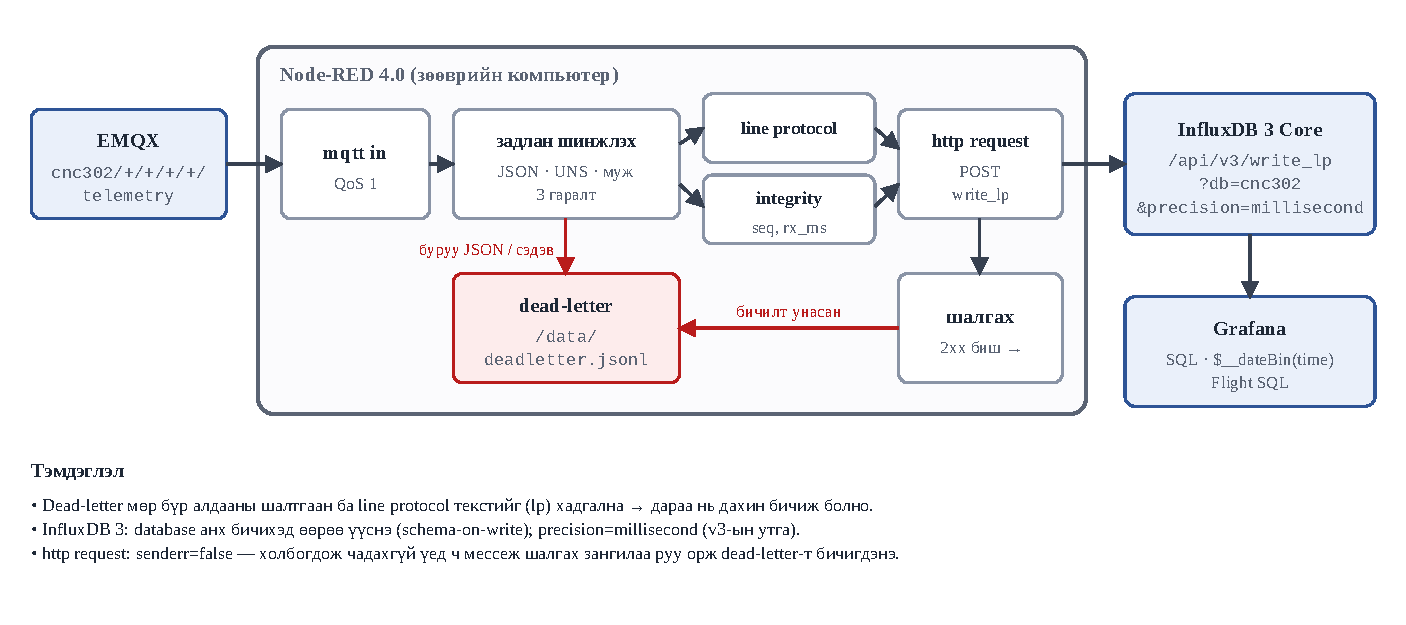
\includegraphics{figures/fig-pipeline.pdf}
\caption{Зураг 5.1 --- Өгөгдлийн шугам: EMQX → Node-RED (parse/validate → line protocol → HTTP write\_lp) → InfluxDB 3 → Grafana, алдаатай мессеж dead-letter файл руу}
\end{figure}

\begin{verbatim}
mqtt in ─▶ задлах + шалгах ─┬─(1)─▶ line protocol (telemetry) ─┐
                            │  └──▶ 60с цонх ─▶ lp (нэгтгэл) ──┤
                            ├─(2)─▶ lp (integrity, rx_ms) ─────┼─▶ InfluxDB бичих ─▶ шалгах ─┬─▶ ok
                            └─(3)─▶ dead-letter ◀──────────────┘                            └─▶ dead-letter
\end{verbatim}

\texttt{data\_\allowbreak{}integrity.\allowbreak{}py}-ийн мессеж (\texttt{run\_id}, \texttt{seq} талбартай) 2-р салаагаар \texttt{integrity} хүснэгтэд бичигдэнэ. Node-RED хүлээн авсан цаг \texttt{rx\_ms} нь MTTR-ыг тооцоход хэрэглэгдэнэ.

\textbf{2.2 Хоёр зангилааг шалга.} \texttt{mqtt-broker} нь \texttt{emqx:1883} (compose сүлжээн доторх нэр, \texttt{localhost} \textbf{биш}), MQTT v5, \texttt{cleansession} унтраалттай, \texttt{sessionExpiry} 3600 с --- Node-RED дахин асахад EMQX хүлээлгэсэн мессежийг өгнө. \texttt{http\ request} нь \texttt{POST\ http:\allowbreak{}/\allowbreak{}/\allowbreak{}influxdb:\allowbreak{}8181/\allowbreak{}api/\allowbreak{}v3/\allowbreak{}write\_\allowbreak{}lp?\allowbreak{}db=\allowbreak{}cnc302\&\allowbreak{}precision=\allowbreak{}millisecond}. Түүний \textbf{"Only send non-2xx responses to Catch node"} сонголт \textbf{унтраалттай} байх ёстой: асаалттай бол InfluxDB унтарсан үеийн холболтын алдаа (\texttt{ECONNREFUSED}) гаралт руу гарахгүй, dead-letter хэзээ ч бичигдэхгүй. Захиалж буй сэдэв: \texttt{cnc302/\allowbreak{}+/\allowbreak{}+/\allowbreak{}+/\allowbreak{}+/\allowbreak{}telemetry}. Dead-letter файл \texttt{/\allowbreak{}data/\allowbreak{}deadletter.\allowbreak{}jsonl} --- \texttt{nodered/node-red} дүрсийн хэрэглэгчийн хавтас \texttt{/data} бөгөөд \texttt{nodered-data} volume-д хадгалагдана.

\textbf{2.3 Өгөгдөл урсгана.} {[}Pi{]} Pi дээр агентаа ажиллуулаад (\texttt{cd\ \textasciitilde{}/cnc302/edge\ \&\&\ make\ agent}), {[}ЗК{]} дээр симулятороор нэмэлт ачаалал өгнө. Node-RED-ийн debug самбарт 10 секунд тутам \texttt{write\_ok} өсөх ёстой:

\begin{Shaded}
\begin{Highlighting}[]
\BuiltInTok{cd}\NormalTok{ \textasciitilde{}/cnc302 }\KeywordTok{\&\&} \ExtensionTok{python3}\NormalTok{ tools/sim\_device.py {-}{-}target cloud {-}{-}host localhost {-}{-}devices 10 {-}{-}interval 1}
\end{Highlighting}
\end{Shaded}

\textbf{2.4 Задлах зангилааны гурван үүрэг} (кодыг нээж уншина):

\begingroup\scriptsize\begin{longtable}[]{@{}lll@{}}
\toprule
\begin{minipage}[b]{0.30\columnwidth}\raggedright
Үүрэг\strut
\end{minipage} & \begin{minipage}[b]{0.30\columnwidth}\raggedright
Код дотор\strut
\end{minipage} & \begin{minipage}[b]{0.30\columnwidth}\raggedright
Яагаад\strut
\end{minipage}\tabularnewline
\midrule
\endhead
\begin{minipage}[t]{0.30\columnwidth}\raggedright
UNS схемийн шалгалт\strut
\end{minipage} & \begin{minipage}[t]{0.30\columnwidth}\raggedright
\texttt{if\ (p.\allowbreak{}length\ !=\allowbreak{}=\allowbreak{}\ 6)}\strut
\end{minipage} & \begin{minipage}[t]{0.30\columnwidth}\raggedright
буруу нэршилтэй өгөгдөл санд орохгүй → dead-letter (\texttt{uns})\strut
\end{minipage}\tabularnewline
\begin{minipage}[t]{0.30\columnwidth}\raggedright
Өгөгдлийн чанар\strut
\end{minipage} & \begin{minipage}[t]{0.30\columnwidth}\raggedright
\texttt{temperature} / \texttt{proc\_\allowbreak{}temp\_\allowbreak{}c} \texttt{\textless{}\ -60\ \textbackslash{}\textbar{}\textbackslash{}\textbar{}\ \textgreater{}\ 150}\strut
\end{minipage} & \begin{minipage}[t]{0.30\columnwidth}\raggedright
эвдэрсэн мэдрэгч нэгтгэлийг сүйтгэнэ → dead-letter (\texttt{range:\ldots{}})\strut
\end{minipage}\tabularnewline
\begin{minipage}[t]{0.30\columnwidth}\raggedright
Шошго гаргах\strut
\end{minipage} & \begin{minipage}[t]{0.30\columnwidth}\raggedright
\texttt{msg.\allowbreak{}tags\ =\allowbreak{}\ \{site,\ area,\ line,\ device\}}\strut
\end{minipage} & \begin{minipage}[t]{0.30\columnwidth}\raggedright
InfluxDB-ийн tag (хэмжээс)\strut
\end{minipage}\tabularnewline
\bottomrule
\end{longtable}\endgroup

Line protocol-д tag утгын \textbf{таслал, тэнцүүгийн тэмдэг, зай}-г \texttt{\textbackslash{}}-ээр escape хийдэг (\texttt{esc()} функц); цаг нь миллисекунд тул URL-д \texttt{precision=\allowbreak{}millisecond}. Ижил хүснэгт + tag set + цагтай хоёр мөр нэг цэг болж нийлдэг тул QoS 1-ийн давхар хүргэлт санд давхар мөр үүсгэхгүй.

\textbf{2.5 Чанарын шүүлт ба dead-letter-ыг туршина:}

\begin{Shaded}
\begin{Highlighting}[]
\CommentTok{\# [ЗК] хүрээнээс гарсан утга — санд ОРОХГҮЙ байх ёстой}
\ExtensionTok{mosquitto\_pub}\NormalTok{ {-}h localhost {-}t }\StringTok{\textquotesingle{}cnc302/shutis/mhts/lab/dev9999/telemetry\textquotesingle{}} \KeywordTok{\textbackslash{}}
  \ExtensionTok{{-}m} \StringTok{\textquotesingle{}\{"ts":\textquotesingle{}"}\VariableTok{$(}\FunctionTok{date}\NormalTok{ +\%s\%3N}\VariableTok{)}\StringTok{"\textquotesingle{},"temperature":9999,"humidity":50,"vibration\_rms":0.3\}\textquotesingle{}}
\ExtensionTok{curl}\NormalTok{ {-}s {-}X POST }\StringTok{\textquotesingle{}http://localhost:8181/api/v3/query\_sql\textquotesingle{}}\NormalTok{ {-}H }\StringTok{\textquotesingle{}Content{-}Type: application/json\textquotesingle{}} \KeywordTok{\textbackslash{}}
  \ExtensionTok{{-}d} \StringTok{\textquotesingle{}\{"db":"cnc302","q":"SELECT count(*) c FROM telemetry WHERE device=\textquotesingle{}"\textquotesingle{}"\textquotesingle{}dev9999\textquotesingle{}"\textquotesingle{}"\textquotesingle{}","format":"json"\}\textquotesingle{}}
\ExtensionTok{docker}\NormalTok{ exec cnc302{-}nodered wc {-}l /data/deadletter.jsonl   \# dead{-}letter файлын урт}
\ExtensionTok{docker}\NormalTok{ exec cnc302{-}nodered tail {-}1 /data/deadletter.jsonl  \# }\DataTypeTok{\{"stage":"parse","reason":"range:temperature",…\}}
\end{Highlighting}
\end{Shaded}

\textbf{2.6 Grafana самбар} (\texttt{:3000}, InfluxDB эх сурвалж аль хэдийн бүртгэгдсэн: query language \textbf{SQL}, database \texttt{cnc302}). SQL горимд Grafana нь InfluxDB 3 руу Flight SQL (gRPC)-ээр холбогддог тул TLS-гүй үед эх сурвалжийн \textbf{Insecure Connection} асаалттай байх ёстой. Гурван панель үүсгэж хадгална --- Алхам 4-д өгсөх урсгал тасрахад энэ график дээр \textbf{цоорхой} үүсэх ёстой (эсвэл үүсэхгүй; аль нь болохыг та хэмжинэ):

\begingroup\scriptsize\begin{longtable}[]{@{}ll@{}}
\toprule
\begin{minipage}[b]{0.47\columnwidth}\raggedright
Панель\strut
\end{minipage} & \begin{minipage}[b]{0.47\columnwidth}\raggedright
Асуулга\strut
\end{minipage}\tabularnewline
\midrule
\endhead
\begin{minipage}[t]{0.47\columnwidth}\raggedright
Температурын цуваа\strut
\end{minipage} & \begin{minipage}[t]{0.47\columnwidth}\raggedright
\texttt{SELECT\ time,\ temperature,\ device\ FROM\ telemetry\ WHERE\ \$\_\allowbreak{}\_\allowbreak{}timeFilter(time)\ ORDER\ BY\ time}\strut
\end{minipage}\tabularnewline
\begin{minipage}[t]{0.47\columnwidth}\raggedright
Идэвхтэй төхөөрөмж (Stat)\strut
\end{minipage} & \begin{minipage}[t]{0.47\columnwidth}\raggedright
\texttt{SELECT\ count(DISTINCT\ device)\ AS\ devices\ FROM\ telemetry\ WHERE\ \$\_\allowbreak{}\_\allowbreak{}timeFilter(time)}\strut
\end{minipage}\tabularnewline
\begin{minipage}[t]{0.47\columnwidth}\raggedright
Бичилтийн хурд\strut
\end{minipage} & \begin{minipage}[t]{0.47\columnwidth}\raggedright
\texttt{SELECT\ \$\_\allowbreak{}\_\allowbreak{}dateBin(time)\ AS\ time,\ count(*)\ AS\ points\ FROM\ telemetry\ WHERE\ \$\_\allowbreak{}\_\allowbreak{}timeFilter(time)\ GROUP\ BY\ 1\ ORDER\ BY\ 1}\strut
\end{minipage}\tabularnewline
\bottomrule
\end{longtable}\endgroup

\texttt{\$\_\allowbreak{}\_\allowbreak{}timeFilter(time)} нь самбарын цагийн хүрээг, \texttt{\$\_\allowbreak{}\_\allowbreak{}dateBin(time)} нь \texttt{date\_bin()}-ийг Grafana-гийн \texttt{\$\_\allowbreak{}\_\allowbreak{}interval}-аар орлуулна. \texttt{GROUP\ BY\ time} (түүхий цагаар бүлэглэх) нь цэг бүрийг тусдаа бүлэг болгодог тул хурдыг харуулахгүй.

\begin{quote}
Албан ёсны баримт: \href{https://grafana.com/docs/grafana/latest/datasources/influxdb/query-editor/}{Grafana --- InfluxDB query editor (SQL macros)}, \href{https://grafana.com/docs/grafana/latest/datasources/influxdb/configure/}{Configure the InfluxDB data source}
\end{quote}

\hypertarget{ux445ux4afux441ux43dux44dux433ux442-5.2-ux448ux443ux433ux430ux43cux44bux43d-ux447ux430ux43dux430ux440ux44bux43d-ux445ux44fux43dux430ux43bux442}{%
\subsubsection{Хүснэгт 5.2 --- Шугамын чанарын хяналт}\label{ux445ux4afux441ux43dux44dux433ux442-5.2-ux448ux443ux433ux430ux43cux44bux43d-ux447ux430ux43dux430ux440ux44bux43d-ux445ux44fux43dux430ux43bux442}}

\begingroup\scriptsize\begin{longtable}[]{@{}ll@{}}
\toprule
Хэмжигдэхүүн & Утга\tabularnewline
\midrule
\endhead
\texttt{write\_ok} (2 минутын дараа) &\tabularnewline
\texttt{write\_errors} &\tabularnewline
Хүрээнээс гарсан утга санд оров уу &\tabularnewline
\texttt{deadletter.jsonl}-ийн мөрийн тоо &\tabularnewline
Grafana дээр өгөгдөл харагдав уу &\tabularnewline
\bottomrule
\end{longtable}\endgroup

\hypertarget{ux430ux43bux445ux430ux43c-3-ux441ux443ux443ux440ux44c-ux431ux4afux440ux44dux43d-ux431ux4afux442ux44dux43d-ux431ux430ux439ux434ux430ux43b-ux433ux4afux4afux440ux44dux44dux440-30-ux43cux438ux43d-piux437ux43a}{%
\subsection{Алхам 3 --- Суурь бүрэн бүтэн байдал: гүүрээр (30 мин) {[}Pi{]}{[}ЗК{]}}\label{ux430ux43bux445ux430ux43c-3-ux441ux443ux443ux440ux44c-ux431ux4afux440ux44dux43d-ux431ux4afux442ux44dux43d-ux431ux430ux439ux434ux430ux43b-ux433ux4afux4afux440ux44dux44dux440-30-ux43cux438ux43d-piux437ux43a}}

Эвдрэлгүй үед \textbf{алдагдал 0\%} байхыг эхлээд батал. Суурь дээр аль хэдийн алдагдаж байвал цааш явах утгагүй.

\begin{Shaded}
\begin{Highlighting}[]
\CommentTok{\# [Pi] терминал 1 — гүүрний төлөвийг бичиж эхэлнэ (ЭНЭ ЦОНХЫГ ЭЦЭС ХҮРТЭЛ БҮҮ ХАА)}
\BuiltInTok{cd}\NormalTok{ \textasciitilde{}/cnc302 }\KeywordTok{\&\&} \FunctionTok{mkdir}\NormalTok{ {-}p lab05/out}
\ExtensionTok{mosquitto\_sub}\NormalTok{ {-}h localhost {-}F }\StringTok{\textquotesingle{}\{"ts":\%U,"state":\%p\}\textquotesingle{}} \KeywordTok{\textbackslash{}}
  \ExtensionTok{{-}t} \StringTok{"cnc302/}\VariableTok{$SITE}\StringTok{/}\VariableTok{$AREA}\StringTok{/}\VariableTok{$LINE}\StringTok{/}\VariableTok{$DEVICE\_ID}\StringTok{/bridge/state"} \OperatorTok{\textgreater{}}\NormalTok{ lab05/out/bridge.jsonl}

\CommentTok{\# [Pi] терминал 2 — ирмэгийн брокер руу нийтэлнэ, гүүр үүл рүү дамжуулна}
\BuiltInTok{cd}\NormalTok{ \textasciitilde{}/cnc302}
\ExtensionTok{python3}\NormalTok{ lab05/data\_integrity.py publish {-}{-}via edge {-}{-}host localhost }\KeywordTok{\textbackslash{}}
    \ExtensionTok{{-}{-}rate}\NormalTok{ 10 {-}{-}seconds 180 {-}{-}qos 1 {-}{-}run{-}id base {-}{-}outdir lab05/out}
\CommentTok{\# дараа нь шалгана — InfluxDB нь ҮҮЛ дээр байгааг санаарай}
\ExtensionTok{python3}\NormalTok{ lab05/data\_integrity.py verify {-}{-}influx }\StringTok{"http://}\VariableTok{$CLOUD\_HOST}\StringTok{:8181"} \KeywordTok{\textbackslash{}}
    \ExtensionTok{{-}{-}run{-}id}\NormalTok{ base {-}{-}outdir lab05/out}
\end{Highlighting}
\end{Shaded}

\begin{quote}
\textbf{Цагийн тохирол.} MTTR-ыг Pi-гийн цаг (тасалдлын цаг) ба зөөврийн компьютерийн цаг (\texttt{rx\_ms}) хоёрыг харьцуулж тооцдог. Хоёр хост дээр \texttt{timedatectl} → \texttt{System\ clock\ synchronized:\allowbreak{}\ yes} байх ёстой.
\end{quote}

\hypertarget{ux445ux4afux441ux43dux44dux433ux442-5.3-ux441ux443ux443ux440ux44c-ux44dux432ux434ux440ux44dux43bux433ux4afux439}{%
\subsubsection{Хүснэгт 5.3 --- Суурь (эвдрэлгүй)}\label{ux445ux4afux441ux43dux44dux433ux442-5.3-ux441ux443ux443ux440ux44c-ux44dux432ux434ux440ux44dux43bux433ux4afux439}}

\begingroup\scriptsize\begin{longtable}[]{@{}ll@{}}
\toprule
Хэмжигдэхүүн & Утга\tabularnewline
\midrule
\endhead
Илгээсэн (амжилттай) &\tabularnewline
Санд олдсон &\tabularnewline
Алдагдал \% & 0.0 байх ЁСТОЙ\tabularnewline
Холболтын тасалдал &\tabularnewline
Хамгийн урт тасалдал (мессеж / сек) & /\tabularnewline
\bottomrule
\end{longtable}\endgroup

\hypertarget{ux430ux43bux445ux430ux43c-4-ux4e9ux433ux441ux4e9ux445-ux443ux440ux441ux433ux430ux43b-uplink-ux442ux430ux441ux440ux430ux445-rpo-ux431ux430-mttr-60-ux43cux438ux43d-piux437ux43a}{%
\subsection{Алхам 4 --- ӨГСӨХ УРСГАЛ (UPLINK) ТАСРАХ: RPO ба MTTR (60 мин) {[}Pi{]}{[}ЗК{]}}\label{ux430ux43bux445ux430ux43c-4-ux4e9ux433ux441ux4e9ux445-ux443ux440ux441ux433ux430ux43b-uplink-ux442ux430ux441ux440ux430ux445-rpo-ux431ux430-mttr-60-ux43cux438ux43d-piux437ux43a}}

\textbf{Энэ бол лабораторийн гол хэсэг.} \texttt{uplink-down} нь Pi → үүл чиглэлийн 1883 портыг л хаана (iptables \texttt{OUTPUT\ \ldots{}\ -j\ DROP}, iptables байхгүй бол nft \texttt{inet\ cnc302} хүснэгт): ирмэгийн mosquitto ажилласаар, төхөөрөмжүүд Pi руу нийтэлсээр байна. Энэ нь "бүх зүйл унасан" биш, яг \textbf{өгсөх урсгал тасарсан} туршилт.

\textbf{4.1 QoS 1, 60 секундын тасалдал.} Гурван терминал зэрэг:

\begin{Shaded}
\begin{Highlighting}[]
\CommentTok{\# [Pi] терминал 1 — bridge.jsonl бичсээр байна (Алхам 3{-}аас үргэлжилнэ)}
\CommentTok{\# [Pi] терминал 2 — 5 минут нийтэлнэ}
\BuiltInTok{cd}\NormalTok{ \textasciitilde{}/cnc302}
\ExtensionTok{python3}\NormalTok{ lab05/data\_integrity.py publish {-}{-}via edge {-}{-}host localhost }\KeywordTok{\textbackslash{}}
    \ExtensionTok{{-}{-}rate}\NormalTok{ 10 {-}{-}seconds 300 {-}{-}qos 1 {-}{-}run{-}id uplink60 {-}{-}outdir lab05/out}
\CommentTok{\# [Pi] терминал 3 — 60 секундын дараа өгсөх урсгалыг 60 секунд таслана}
\FunctionTok{sleep}\NormalTok{ 60 }\KeywordTok{\&\&} \FunctionTok{bash}\NormalTok{ lab05/failure\_inject.sh uplink{-}down 60}
\end{Highlighting}
\end{Shaded}

Энэ үед юу болдгийг Зураг 5.2-оос дахин хар. \texttt{failure\_\allowbreak{}inject.\allowbreak{}sh} тасалдлын эхлэл/төгсгөлийг \texttt{lab05/\allowbreak{}out/\allowbreak{}uplink-events.\allowbreak{}jsonl}-д бичнэ.

\textbf{4.2 Өгсөх урсгал унах үед {[}Pi{]} дээр дараалал өсөж байгааг хар:}

\begin{Shaded}
\begin{Highlighting}[]
\CommentTok{\# хадгалагдсан мессежийн тоо (retained + тогтвортой клиентийн дараалал);}
\CommentTok{\# sys\_interval (анхдагч 10 с) тутам шинэчлэгдэнэ. Хуучин нэр нь $SYS/broker/messages/stored}
\ExtensionTok{mosquitto\_sub}\NormalTok{ {-}h localhost {-}t }\StringTok{\textquotesingle{}$SYS/broker/store/messages/count\textquotesingle{}}\NormalTok{ {-}C 1}
\ExtensionTok{docker}\NormalTok{ stats {-}{-}no{-}stream cnc302{-}mosquitto        \# RAM өсөж байна уу}
\end{Highlighting}
\end{Shaded}

Гүүр тасралтыг хэзээ илрүүлснийг \texttt{bridge.jsonl}-ээс хар --- \texttt{uplink-down}-оос хэдэн секундын дараа \texttt{"state":0} гарав (эсвэл огт гарсангүй)? Энэ зөрүүг Хүснэгт 5.5-д бич.

\begin{quote}
\textbf{Урхинд бүү ор.} Өгсөх урсгал сэргэсний дараа шинэ \texttt{mosquitto\_sub} асаавал дахин илгээгдсэн мессеж \textbf{харагдахгүй} --- тэсрэлт аль хэдийн өнгөрсөн байна. Дахин илгээлтийн нотолгоо нь зөвхөн (а) InfluxDB дэх мөрүүд, (б) Алхам 3-аас хойш тасралтгүй ажиллаж байгаа \texttt{bridge.jsonl} хоёр.
\end{quote}

\textbf{4.3 Шалгах --- алдагдлыг гүүрний төлөвөөр ХУВААНА:}

\begin{Shaded}
\begin{Highlighting}[]
\CommentTok{\# [Pi] publish дуусмагц (сэргэхийг 30 сек хүлээгээд)}
\ExtensionTok{python3}\NormalTok{ lab05/data\_integrity.py verify {-}{-}influx }\StringTok{"http://}\VariableTok{$CLOUD\_HOST}\StringTok{:8181"} \KeywordTok{\textbackslash{}}
    \ExtensionTok{{-}{-}run{-}id}\NormalTok{ uplink60 {-}{-}outdir lab05/out {-}{-}bridge{-}log lab05/out/bridge.jsonl }\KeywordTok{\textbackslash{}}
    \ExtensionTok{{-}{-}cut{-}log}\NormalTok{ lab05/out/uplink{-}events.jsonl}
\end{Highlighting}
\end{Shaded}

Гаралт нь алдагдлыг хоёр янзаар хуваана: (а) \textbf{гүүрийн мэдээлсэн} төлөвөөр (\texttt{-\/-bridge-log}), (б) \textbf{бодит} тасалдлаар (\texttt{-\/-cut-log}), мөн MTTR-ыг автоматаар тооцно. Хоёр хуваалтын "тасарсан (с)" ялгаа нь гүүрийн илрүүлэх хугацаа юм.

\textbf{4.4 QoS 0-оор давт} (шинэ \texttt{-\/-run-id}, ижил хэв маяг):

\begin{Shaded}
\begin{Highlighting}[]
\ExtensionTok{python3}\NormalTok{ lab05/data\_integrity.py publish {-}{-}via edge {-}{-}host localhost }\KeywordTok{\textbackslash{}}
    \ExtensionTok{{-}{-}rate}\NormalTok{ 10 {-}{-}seconds 300 {-}{-}qos 0 {-}{-}run{-}id uplink60q0 {-}{-}outdir lab05/out}
\CommentTok{\# 60 сек дараа: bash lab05/failure\_inject.sh uplink{-}down 60 ; дараа нь:}
\ExtensionTok{python3}\NormalTok{ lab05/data\_integrity.py verify {-}{-}influx }\StringTok{"http://}\VariableTok{$CLOUD\_HOST}\StringTok{:8181"} \KeywordTok{\textbackslash{}}
    \ExtensionTok{{-}{-}run{-}id}\NormalTok{ uplink60q0 {-}{-}outdir lab05/out {-}{-}bridge{-}log lab05/out/bridge.jsonl }\KeywordTok{\textbackslash{}}
    \ExtensionTok{{-}{-}cut{-}log}\NormalTok{ lab05/out/uplink{-}events.jsonl}
\end{Highlighting}
\end{Shaded}

\textbf{4.5 Тасалдлыг уртасга:} ижил туршилтыг \texttt{uplink-down\ 180} (3 минут) -аар давт (\texttt{-\/-seconds\ 420}, \texttt{-\/\allowbreak{}-run-id\ uplink180}).

\hypertarget{ux445ux4afux441ux43dux44dux433ux442-5.4-ux4e9ux433ux441ux4e9ux445-ux443ux440ux441ux433ux430ux43b-ux442ux430ux441ux440ux430ux445-rpo-ux431ux430-mttr}{%
\subsubsection{Хүснэгт 5.4 --- Өгсөх урсгал тасрах: RPO ба MTTR}\label{ux445ux4afux441ux43dux44dux433ux442-5.4-ux4e9ux433ux441ux4e9ux445-ux443ux440ux441ux433ux430ux43b-ux442ux430ux441ux440ux430ux445-rpo-ux431ux430-mttr}}

\begingroup\scriptsize\begin{longtable}[]{@{}lllllllll@{}}
\toprule
\begin{minipage}[b]{0.08\columnwidth}\raggedright
Ажиллалт\strut
\end{minipage} & \begin{minipage}[b]{0.08\columnwidth}\raggedright
QoS\strut
\end{minipage} & \begin{minipage}[b]{0.08\columnwidth}\raggedright
Тасалдал (с)\strut
\end{minipage} & \begin{minipage}[b]{0.08\columnwidth}\raggedright
Илгээсэн\strut
\end{minipage} & \begin{minipage}[b]{0.08\columnwidth}\raggedright
Санд хүрсэн\strut
\end{minipage} & \begin{minipage}[b]{0.08\columnwidth}\raggedright
Алдагдал \%\strut
\end{minipage} & \begin{minipage}[b]{0.08\columnwidth}\raggedright
\textbf{RPO (с)}\strut
\end{minipage} & \begin{minipage}[b]{0.08\columnwidth}\raggedright
\textbf{MTTR (с)}\strut
\end{minipage} & \begin{minipage}[b]{0.08\columnwidth}\raggedright
Гүүр дахин холбогдох хугацаа (с)\strut
\end{minipage}\tabularnewline
\midrule
\endhead
\begin{minipage}[t]{0.08\columnwidth}\raggedright
\texttt{uplink60}\strut
\end{minipage} & \begin{minipage}[t]{0.08\columnwidth}\raggedright
1\strut
\end{minipage} & \begin{minipage}[t]{0.08\columnwidth}\raggedright
60\strut
\end{minipage} & \begin{minipage}[t]{0.08\columnwidth}\raggedright
\strut
\end{minipage} & \begin{minipage}[t]{0.08\columnwidth}\raggedright
\strut
\end{minipage} & \begin{minipage}[t]{0.08\columnwidth}\raggedright
\strut
\end{minipage} & \begin{minipage}[t]{0.08\columnwidth}\raggedright
\strut
\end{minipage} & \begin{minipage}[t]{0.08\columnwidth}\raggedright
\strut
\end{minipage} & \begin{minipage}[t]{0.08\columnwidth}\raggedright
\strut
\end{minipage}\tabularnewline
\begin{minipage}[t]{0.08\columnwidth}\raggedright
\texttt{uplink60q0}\strut
\end{minipage} & \begin{minipage}[t]{0.08\columnwidth}\raggedright
0\strut
\end{minipage} & \begin{minipage}[t]{0.08\columnwidth}\raggedright
60\strut
\end{minipage} & \begin{minipage}[t]{0.08\columnwidth}\raggedright
\strut
\end{minipage} & \begin{minipage}[t]{0.08\columnwidth}\raggedright
\strut
\end{minipage} & \begin{minipage}[t]{0.08\columnwidth}\raggedright
\strut
\end{minipage} & \begin{minipage}[t]{0.08\columnwidth}\raggedright
\strut
\end{minipage} & \begin{minipage}[t]{0.08\columnwidth}\raggedright
\strut
\end{minipage} & \begin{minipage}[t]{0.08\columnwidth}\raggedright
\strut
\end{minipage}\tabularnewline
\begin{minipage}[t]{0.08\columnwidth}\raggedright
\texttt{uplink180}\strut
\end{minipage} & \begin{minipage}[t]{0.08\columnwidth}\raggedright
1\strut
\end{minipage} & \begin{minipage}[t]{0.08\columnwidth}\raggedright
180\strut
\end{minipage} & \begin{minipage}[t]{0.08\columnwidth}\raggedright
\strut
\end{minipage} & \begin{minipage}[t]{0.08\columnwidth}\raggedright
\strut
\end{minipage} & \begin{minipage}[t]{0.08\columnwidth}\raggedright
\strut
\end{minipage} & \begin{minipage}[t]{0.08\columnwidth}\raggedright
\strut
\end{minipage} & \begin{minipage}[t]{0.08\columnwidth}\raggedright
\strut
\end{minipage} & \begin{minipage}[t]{0.08\columnwidth}\raggedright
\strut
\end{minipage}\tabularnewline
\bottomrule
\end{longtable}\endgroup

\begin{itemize}
\tightlist
\item
  \textbf{RPO} = хамгийн урт тасалдлын хугацаа (\texttt{verify}-ийн "Хамгийн урт тасалдал ... секунд"). Алдагдал 0 бол RPO = 0.
\item
  \textbf{MTTR} = өгсөх урсгал сэргэснээс (\texttt{uplink-events.\allowbreak{}jsonl}-ийн \texttt{state=1}) тасалдлын үеэр илгээсэн сүүлийн мессеж санд хүрэх (\texttt{integrity.rx\_ms}) хүртэлх хугацаа --- \texttt{verify\ -\/\allowbreak{}-cut-log} хэвлэнэ (\texttt{mttr\_s}).
\item
  \textbf{Гүүр дахин холбогдох хугацаа} = \texttt{bridge.jsonl}-ийн \texttt{state=1} − \texttt{uplink-events.\allowbreak{}jsonl}-ийн \texttt{state=1}.
\end{itemize}

\hypertarget{ux445ux4afux441ux43dux44dux433ux442-5.5-ux431ux43eux434ux438ux442-ux442ux430ux441ux430ux43bux434ux430ux43b-ux431ux430-ux433ux4afux4afux440ux438ux439ux43d-ux43cux44dux434ux44dux44dux43bux441ux44dux43d-ux442ux4e9ux43bux4e9ux432ux4e9ux4e9ux440-ux445ux443ux432ux430ux430ux441ux430ux43d-ux430ux43bux434ux430ux433ux434ux430ux43b---cut-log---bridge-log}{%
\subsubsection{\texorpdfstring{Хүснэгт 5.5 --- Бодит тасалдал ба гүүрийн мэдээлсэн төлөвөөр хуваасан алдагдал (\texttt{-\/-cut-log}, \texttt{-\/-bridge-log})}{Хүснэгт 5.5 --- Бодит тасалдал ба гүүрийн мэдээлсэн төлөвөөр хуваасан алдагдал (-\/-cut-log, -\/-bridge-log)}}\label{ux445ux4afux441ux43dux44dux433ux442-5.5-ux431ux43eux434ux438ux442-ux442ux430ux441ux430ux43bux434ux430ux43b-ux431ux430-ux433ux4afux4afux440ux438ux439ux43d-ux43cux44dux434ux44dux44dux43bux441ux44dux43d-ux442ux4e9ux43bux4e9ux432ux4e9ux4e9ux440-ux445ux443ux432ux430ux430ux441ux430ux43d-ux430ux43bux434ux430ux433ux434ux430ux43b---cut-log---bridge-log}}

\begingroup\scriptsize\begin{longtable}[]{@{}llllll@{}}
\toprule
\begin{minipage}[b]{0.14\columnwidth}\raggedright
Ажиллалт\strut
\end{minipage} & \begin{minipage}[b]{0.14\columnwidth}\raggedright
Бодит тасалдал (с, \texttt{-\/-cut-log})\strut
\end{minipage} & \begin{minipage}[b]{0.14\columnwidth}\raggedright
Гүүрийн мэдээлсэн тасалдал (с, \texttt{-\/-bridge-log})\strut
\end{minipage} & \begin{minipage}[b]{0.14\columnwidth}\raggedright
Илрүүлэх хугацаа (с)\strut
\end{minipage} & \begin{minipage}[b]{0.14\columnwidth}\raggedright
Бодит тасалдлын үед: илгээсэн / алдагдсан / \%\strut
\end{minipage} & \begin{minipage}[b]{0.14\columnwidth}\raggedright
Ажиллаж байхад: илгээсэн / алдагдсан / \%\strut
\end{minipage}\tabularnewline
\midrule
\endhead
\begin{minipage}[t]{0.14\columnwidth}\raggedright
\texttt{uplink60} (QoS 1)\strut
\end{minipage} & \begin{minipage}[t]{0.14\columnwidth}\raggedright
\strut
\end{minipage} & \begin{minipage}[t]{0.14\columnwidth}\raggedright
\strut
\end{minipage} & \begin{minipage}[t]{0.14\columnwidth}\raggedright
\strut
\end{minipage} & \begin{minipage}[t]{0.14\columnwidth}\raggedright
/ /\strut
\end{minipage} & \begin{minipage}[t]{0.14\columnwidth}\raggedright
/ /\strut
\end{minipage}\tabularnewline
\begin{minipage}[t]{0.14\columnwidth}\raggedright
\texttt{uplink60q0} (QoS 0)\strut
\end{minipage} & \begin{minipage}[t]{0.14\columnwidth}\raggedright
\strut
\end{minipage} & \begin{minipage}[t]{0.14\columnwidth}\raggedright
\strut
\end{minipage} & \begin{minipage}[t]{0.14\columnwidth}\raggedright
\strut
\end{minipage} & \begin{minipage}[t]{0.14\columnwidth}\raggedright
/ /\strut
\end{minipage} & \begin{minipage}[t]{0.14\columnwidth}\raggedright
/ /\strut
\end{minipage}\tabularnewline
\begin{minipage}[t]{0.14\columnwidth}\raggedright
\texttt{uplink180} (QoS 1)\strut
\end{minipage} & \begin{minipage}[t]{0.14\columnwidth}\raggedright
\strut
\end{minipage} & \begin{minipage}[t]{0.14\columnwidth}\raggedright
\strut
\end{minipage} & \begin{minipage}[t]{0.14\columnwidth}\raggedright
\strut
\end{minipage} & \begin{minipage}[t]{0.14\columnwidth}\raggedright
/ /\strut
\end{minipage} & \begin{minipage}[t]{0.14\columnwidth}\raggedright
/ /\strut
\end{minipage}\tabularnewline
\bottomrule
\end{longtable}\endgroup

\begin{quote}
\textbf{Хүлээгдэх үр дүн:} \texttt{cleansession\ false} + \texttt{local\_\allowbreak{}cleansession\ false} + \texttt{queue\_\allowbreak{}qos0\_\allowbreak{}messages\ true} үед \textbf{QoS 1}-ийн алдагдал 0\% байх ёстой --- PUBACK аваагүй мессеж session-д үлдэж, дахин холбогдоход илгээгдэнэ. \textbf{QoS 0}-д гүүр тасралтыг илрүүлэхээс өмнө TCP руу бичигдсэн мессеж алдагдаж болно (§3, 2-р зүйл) --- алдагдсан хэсэг тасалдлын \textbf{эхэнд} байвал яг энэ шалтгаан. 60 секундын тасалдалд гүүр "0" мэдээлээгүй байж болохыг анхаар (keepalive 60 с).
\end{quote}

\hypertarget{ux430ux43bux445ux430ux43c-5-cleansession-ux431ux430-ux434ux430ux440ux430ux430ux43bux43bux44bux43d-ux445ux44fux437ux433ux430ux430ux440-35-ux43cux438ux43d-pi}{%
\subsection{\texorpdfstring{Алхам 5 --- \texttt{cleansession} ба дарааллын хязгаар (35 мин) {[}Pi{]}}{Алхам 5 --- cleansession ба дарааллын хязгаар (35 мин) {[}Pi{]}}}\label{ux430ux43bux445ux430ux43c-5-cleansession-ux431ux430-ux434ux430ux440ux430ux430ux43bux43bux44bux43d-ux445ux44fux437ux433ux430ux430ux440-35-ux43cux438ux43d-pi}}

\textbf{5.1 \texttt{cleansession} ба \texttt{local\_\allowbreak{}cleansession}-ийг салгаж турш.} \texttt{bridge.conf}-д \texttt{local\_\allowbreak{}cleansession\ false} \textbf{ил} бичигдсэн тул зөвхөн \texttt{cleansession}-ийг \texttt{true} болгох нь гүүрний \textbf{локал} дарааллыг хөндөхгүй --- энэ хоёрын үүргийг ялгах нь энэ алхмын зорилго. Гүүрний тохиргоог \textbf{шууд} засаад Алхам 4.1-ийг хоёр удаа давтана:

\begin{Shaded}
\begin{Highlighting}[]
\BuiltInTok{cd}\NormalTok{ \textasciitilde{}/cnc302/edge}
\CommentTok{\# (а) зөвхөн алсын тал цэвэр:  cleansession true,  local\_cleansession false  → {-}{-}run{-}id uplink60clean}
\CommentTok{\# (б) хоёр тал цэвэр:          cleansession true,  local\_cleansession true   → {-}{-}run{-}id uplink60cleanboth}
\FunctionTok{nano}\NormalTok{ mosquitto/conf.d/bridge.conf}
\ExtensionTok{docker}\NormalTok{ compose restart mosquitto      \# ⚠ }\KeywordTok{\textasciigrave{}}\FunctionTok{make}\NormalTok{ restart}\KeywordTok{\textasciigrave{}}\NormalTok{ БИШ!}
\ExtensionTok{docker}\NormalTok{ compose logs {-}{-}tail=20 mosquitto }\KeywordTok{|} \FunctionTok{grep}\NormalTok{ {-}i bridge}
\end{Highlighting}
\end{Shaded}

\begin{quote}
Бидний урьдчилсан туршилтаар (mosquitto 2.0, QoS 1, 30 с тасалдал) (а) алдагдалгүй, (б) тасалдлын үеийн мессеж бараг бүгд алдагдсан. Өөрсдийн тоогоор батал.
\end{quote}

\begin{quote}
⚠ \texttt{make\ restart} нь эхлээд \texttt{make\ bridge}-ийг ажиллуулж \texttt{bridge.conf}-ыг \textbf{загвараас дахин үүсгэдэг} --- гар засвар устана. Тиймээс энд \texttt{docker\ compose\ restart\ mosquitto}. Дуусаад \texttt{make\ bridge}-ээр анхны төлөвт буцаана.
\end{quote}

\textbf{5.2 Дарааллын RAM-ын арифметик.} \texttt{mosquitto.conf} дахь \texttt{max\_\allowbreak{}queued\_\allowbreak{}messages\ 100000} юу гэсэн үг вэ --- тоол:

\begin{verbatim}
100 000 мессеж × ______ Б (таны ачаалал) = ______ MiB
Pi-гийн боломжтой RAM (Лаб 4, Хүснэгт 4.1) = ______ MiB
→ Дараалал бүрэн дүүрэхэд Pi амьд үлдэх үү: ______
→ Таны хурдаар (______ мсж/с) дараалал дүүрэхэд ______ секунд шаардагдана
\end{verbatim}

\textbf{5.3 Дарааллын халилтыг үзэх.} Хязгаарыг зориудаар багасгаж, халихыг ажигла. \texttt{max\_\allowbreak{}queued\_\allowbreak{}messages} нь "дамжуулж байгаа (in-flight) мессежээс \textbf{гадна}" хадгалах QoS 1/2 мессежийн тоо (клиент тус бүрд):

\begin{Shaded}
\begin{Highlighting}[]
\BuiltInTok{cd}\NormalTok{ \textasciitilde{}/cnc302/edge}
\FunctionTok{sed}\NormalTok{ {-}i }\StringTok{\textquotesingle{}s/\^{}max\_queued\_messages .*/max\_queued\_messages 500/\textquotesingle{}}\NormalTok{ mosquitto/mosquitto.conf}
\ExtensionTok{docker}\NormalTok{ compose restart mosquitto}
\CommentTok{\# [Pi] өөр терминалд: 120 сек тасалж, 10 мсж/с илгээнэ → 1200 мессеж \textgreater{} 500 дараалал}
\BuiltInTok{cd}\NormalTok{ \textasciitilde{}/cnc302}
\ExtensionTok{python3}\NormalTok{ lab05/data\_integrity.py publish {-}{-}via edge {-}{-}host localhost }\KeywordTok{\textbackslash{}}
    \ExtensionTok{{-}{-}rate}\NormalTok{ 10 {-}{-}seconds 240 {-}{-}qos 1 {-}{-}run{-}id qfull {-}{-}outdir lab05/out}
\CommentTok{\# 30 сек дараа: bash lab05/failure\_inject.sh uplink{-}down 120 ; дараа нь:}
\ExtensionTok{python3}\NormalTok{ lab05/data\_integrity.py verify {-}{-}influx }\StringTok{"http://}\VariableTok{$CLOUD\_HOST}\StringTok{:8181"} \KeywordTok{\textbackslash{}}
    \ExtensionTok{{-}{-}run{-}id}\NormalTok{ qfull {-}{-}outdir lab05/out {-}{-}bridge{-}log lab05/out/bridge.jsonl }\KeywordTok{\textbackslash{}}
    \ExtensionTok{{-}{-}cut{-}log}\NormalTok{ lab05/out/uplink{-}events.jsonl}
\ExtensionTok{docker}\NormalTok{ compose {-}f \textasciitilde{}/cnc302/edge/docker{-}compose.yml logs mosquitto }\KeywordTok{|} \FunctionTok{grep}\NormalTok{ {-}i }\StringTok{"dropped"}
\CommentTok{\# Дуусаад БУЦААЖ 100000 болгоод дахин асаана}
\end{Highlighting}
\end{Shaded}

Алдагдсан \texttt{seq}-ийн хүрээ тасалдлын \textbf{эхэнд} үү, \textbf{төгсгөлд} үү гэдгийг \texttt{verify}-ийн тасралтын жагсаалтаас ол.

\hypertarget{ux445ux4afux441ux43dux44dux433ux442-5.6-cleansession-ux431ux430-ux434ux430ux440ux430ux430ux43bux43bux44bux43d-ux445ux44fux437ux433ux430ux430ux440ux44bux43d-ux445ux430ux440ux44cux446ux443ux443ux43bux430ux43bux442}{%
\subsubsection{\texorpdfstring{Хүснэгт 5.6 --- \texttt{cleansession} ба дарааллын хязгаарын харьцуулалт}{Хүснэгт 5.6 --- cleansession ба дарааллын хязгаарын харьцуулалт}}\label{ux445ux4afux441ux43dux44dux433ux442-5.6-cleansession-ux431ux430-ux434ux430ux440ux430ux430ux43bux43bux44bux43d-ux445ux44fux437ux433ux430ux430ux440ux44bux43d-ux445ux430ux440ux44cux446ux443ux443ux43bux430ux43bux442}}

\begingroup\scriptsize\begin{longtable}[]{@{}lllll@{}}
\toprule
\begin{minipage}[b]{0.17\columnwidth}\raggedright
Тохиргоо\strut
\end{minipage} & \begin{minipage}[b]{0.17\columnwidth}\raggedright
Гүүр унасан үед илгээсэн\strut
\end{minipage} & \begin{minipage}[b]{0.17\columnwidth}\raggedright
Алдагдсан\strut
\end{minipage} & \begin{minipage}[b]{0.17\columnwidth}\raggedright
Алдагдал \%\strut
\end{minipage} & \begin{minipage}[b]{0.17\columnwidth}\raggedright
Дараалал хадгалагдав уу\strut
\end{minipage}\tabularnewline
\midrule
\endhead
\begin{minipage}[t]{0.17\columnwidth}\raggedright
\texttt{cleansession\ false}, \texttt{local\_\allowbreak{}cleansession\ false}, дараалал 100000 (үндсэн)\strut
\end{minipage} & \begin{minipage}[t]{0.17\columnwidth}\raggedright
\strut
\end{minipage} & \begin{minipage}[t]{0.17\columnwidth}\raggedright
\strut
\end{minipage} & \begin{minipage}[t]{0.17\columnwidth}\raggedright
\strut
\end{minipage} & \begin{minipage}[t]{0.17\columnwidth}\raggedright
\strut
\end{minipage}\tabularnewline
\begin{minipage}[t]{0.17\columnwidth}\raggedright
\texttt{cleansession\ true}, \texttt{local\_\allowbreak{}cleansession\ false}, дараалал 100000\strut
\end{minipage} & \begin{minipage}[t]{0.17\columnwidth}\raggedright
\strut
\end{minipage} & \begin{minipage}[t]{0.17\columnwidth}\raggedright
\strut
\end{minipage} & \begin{minipage}[t]{0.17\columnwidth}\raggedright
\strut
\end{minipage} & \begin{minipage}[t]{0.17\columnwidth}\raggedright
\strut
\end{minipage}\tabularnewline
\begin{minipage}[t]{0.17\columnwidth}\raggedright
\texttt{cleansession\ true}, \texttt{local\_\allowbreak{}cleansession\ true}, дараалал 100000\strut
\end{minipage} & \begin{minipage}[t]{0.17\columnwidth}\raggedright
\strut
\end{minipage} & \begin{minipage}[t]{0.17\columnwidth}\raggedright
\strut
\end{minipage} & \begin{minipage}[t]{0.17\columnwidth}\raggedright
\strut
\end{minipage} & \begin{minipage}[t]{0.17\columnwidth}\raggedright
\strut
\end{minipage}\tabularnewline
\begin{minipage}[t]{0.17\columnwidth}\raggedright
\texttt{cleansession\ false}, дараалал 500\strut
\end{minipage} & \begin{minipage}[t]{0.17\columnwidth}\raggedright
\strut
\end{minipage} & \begin{minipage}[t]{0.17\columnwidth}\raggedright
\strut
\end{minipage} & \begin{minipage}[t]{0.17\columnwidth}\raggedright
\strut
\end{minipage} & \begin{minipage}[t]{0.17\columnwidth}\raggedright
\strut
\end{minipage}\tabularnewline
\bottomrule
\end{longtable}\endgroup

\hypertarget{ux445ux4afux441ux43dux44dux433ux442-5.7-ux434ux430ux440ux430ux430ux43bux43bux44bux43d-ux43dux4e9ux4e9ux446ux438ux439ux43d-ux437ux430ux440ux434ux430ux43b}{%
\subsubsection{Хүснэгт 5.7 --- Дарааллын нөөцийн зардал}\label{ux445ux4afux441ux43dux44dux433ux442-5.7-ux434ux430ux440ux430ux430ux43bux43bux44bux43d-ux43dux4e9ux4e9ux446ux438ux439ux43d-ux437ux430ux440ux434ux430ux43b}}

\begingroup\scriptsize\begin{longtable}[]{@{}ll@{}}
\toprule
Асуулт & Хариулт\tabularnewline
\midrule
\endhead
Нэг мессежийн бодит хэмжээ (Б) &\tabularnewline
100 000 мессежийн RAM (MiB) &\tabularnewline
Дараалал дүүрэх хугацаа таны хурдаар (с) &\tabularnewline
Дараалал өсөх үед mosquitto-гийн RAM хэдээр өсөв (MiB) &\tabularnewline
Дараалал халихад аль мессеж хаягдав (хуучин уу, шинэ үү) &\tabularnewline
\bottomrule
\end{longtable}\endgroup

\textbf{5.4 microSD-гийн бичих саатал.} mosquitto-гийн persistence ба InfluxDB хоёулаа диск рүү бичдэг. Pi-гийн картыг хэмж (4 KiB × 2000 синхрон бичилт):

\begin{Shaded}
\begin{Highlighting}[]
\FunctionTok{dd}\NormalTok{ if=/dev/zero of=\textasciitilde{}/cnc302/sdtest bs=4k count=2000 oflag=dsync }\OperatorTok{2\textgreater{}\&1} \KeywordTok{|} \FunctionTok{tail}\NormalTok{ {-}1}
\FunctionTok{rm}\NormalTok{ \textasciitilde{}/cnc302/sdtest }\KeywordTok{\&\&} \FunctionTok{vmstat}\NormalTok{ 1 5      \# }\KeywordTok{\textasciigrave{}}\ExtensionTok{wa}\KeywordTok{\textasciigrave{}}\NormalTok{ = I/O хүлээлт}
\end{Highlighting}
\end{Shaded}

Гарсан тоог \texttt{autosave\_\allowbreak{}interval\ 60}-той холбож тайлбарла: mosquitto яагаад бичилт бүрийг шууд диск рүү буулгадаггүй вэ, энэ нь тасалдал үед юу алдах эрсдэлтэй вэ? Хариултаа Алхам 6-гийн \texttt{broker} (хэвийн зогсоолт → \texttt{mosquitto.db} бичигдэнэ) ба \texttt{broker-kill} (SIGKILL → бичигдэхгүй) хоёрын үр дүнгээр батал.

\hypertarget{ux430ux43bux445ux430ux43c-6-ux431ux443ux441ux430ux434-ux44dux432ux434ux440ux44dux43bux4afux4afux434-30-ux43cux438ux43d-piux437ux43a}{%
\subsection{Алхам 6 --- Бусад эвдрэлүүд (30 мин) {[}Pi{]}{[}ЗК{]}}\label{ux430ux43bux445ux430ux43c-6-ux431ux443ux441ux430ux434-ux44dux432ux434ux440ux44dux43bux4afux4afux434-30-ux43cux438ux43d-piux437ux43a}}

Тус бүрд \texttt{publish} ажиллаж байх зуур эвдрэлийг үүсгэнэ (60 секундын дараа), дараа нь \texttt{verify}.

\begin{Shaded}
\begin{Highlighting}[]
\CommentTok{\# [Pi] ирмэгийн брокер өөрөө унана — гүүр биш, БРОКЕР (хэвийн SIGTERM → mosquitto.db хадгалагдана)}
\FunctionTok{bash}\NormalTok{ lab05/failure\_inject.sh broker 30}
\CommentTok{\# [Pi] цахилгаан тасрахыг дуурайна: өгсөх урсгал тасарсан ҮЕД mosquitto{-}г SIGKILL{-}ээр унагана}
\CommentTok{\#    (терминал 3: uplink{-}down 120 ажиллаж байх үед 40 сек дараа)}
\FunctionTok{bash}\NormalTok{ lab05/failure\_inject.sh broker{-}kill 20}
\CommentTok{\# [ЗК] ҮҮЛ дээр: InfluxDB унана. Брокер, гүүр ажилласаар байна!}
\FunctionTok{bash}\NormalTok{ lab05/failure\_inject.sh influx 30}
\ExtensionTok{docker}\NormalTok{ exec cnc302{-}nodered wc {-}l /data/deadletter.jsonl    \# dead{-}letter ажиллав уу}
\CommentTok{\# [Pi] CPU ханалт (дулааны төсөв ч мөн шалгагдана)}
\FunctionTok{bash}\NormalTok{ lab05/failure\_inject.sh cpu 45}
\CommentTok{\# [Pi] АЮУЛГҮЙ дискний туршилт — /dev/shm (RAM) дээрх 64 MiB loop файл, бодит microSD хөндөгдөхгүй}
\FunctionTok{bash}\NormalTok{ lab05/failure\_inject.sh disk 60}
\CommentTok{\# Эцэст нь БҮГДИЙГ сэргээнэ}
\FunctionTok{bash}\NormalTok{ lab05/failure\_inject.sh restore}
\end{Highlighting}
\end{Shaded}

\begin{quote}
\texttt{influx} горим нь хамгийн заль мэхтэй тохиолдол: \textbf{төхөөрөмж юу ч анзаарахгүй}, брокер хүлээж авсаар байна, гүүр ажиллаж байна --- гэвч өгөгдөл хаана ч хадгалагдахгүй. Ийм эвдрэлийг зөвхөн Node-RED-ийн \texttt{write\_errors} тоолуур ба dead-letter файлаас л илрүүлнэ. Grafana дээр график тасарна --- гэхдээ хэн нэг нь харж байвал л.
\end{quote}

\hypertarget{ux445ux4afux441ux43dux44dux433ux442-5.8-ux44dux432ux434ux440ux44dux43bux438ux439ux43d-ux43cux430ux442ux440ux438ux446}{%
\subsubsection{Хүснэгт 5.8 --- ЭВДРЭЛИЙН МАТРИЦ}\label{ux445ux4afux441ux43dux44dux433ux442-5.8-ux44dux432ux434ux440ux44dux43bux438ux439ux43d-ux43cux430ux442ux440ux438ux446}}

\begingroup\scriptsize\begin{longtable}[]{@{}llllllllll@{}}
\toprule
\begin{minipage}[b]{0.07\columnwidth}\raggedright
\#\strut
\end{minipage} & \begin{minipage}[b]{0.07\columnwidth}\raggedright
Эвдрэл\strut
\end{minipage} & \begin{minipage}[b]{0.07\columnwidth}\raggedright
Үргэлжлэл (с)\strut
\end{minipage} & \begin{minipage}[b]{0.07\columnwidth}\raggedright
Шинж тэмдэг\strut
\end{minipage} & \begin{minipage}[b]{0.07\columnwidth}\raggedright
Илгээсэн\strut
\end{minipage} & \begin{minipage}[b]{0.07\columnwidth}\raggedright
Санд хүрсэн\strut
\end{minipage} & \begin{minipage}[b]{0.07\columnwidth}\raggedright
Алдагдал \%\strut
\end{minipage} & \begin{minipage}[b]{0.07\columnwidth}\raggedright
RPO (с)\strut
\end{minipage} & \begin{minipage}[b]{0.07\columnwidth}\raggedright
MTTR (с)\strut
\end{minipage} & \begin{minipage}[b]{0.07\columnwidth}\raggedright
Автоматаар сэргэв үү\strut
\end{minipage}\tabularnewline
\midrule
\endhead
\begin{minipage}[t]{0.07\columnwidth}\raggedright
0\strut
\end{minipage} & \begin{minipage}[t]{0.07\columnwidth}\raggedright
Суурь (эвдрэлгүй)\strut
\end{minipage} & \begin{minipage}[t]{0.07\columnwidth}\raggedright
---\strut
\end{minipage} & \begin{minipage}[t]{0.07\columnwidth}\raggedright
\strut
\end{minipage} & \begin{minipage}[t]{0.07\columnwidth}\raggedright
\strut
\end{minipage} & \begin{minipage}[t]{0.07\columnwidth}\raggedright
\strut
\end{minipage} & \begin{minipage}[t]{0.07\columnwidth}\raggedright
\strut
\end{minipage} & \begin{minipage}[t]{0.07\columnwidth}\raggedright
\strut
\end{minipage} & \begin{minipage}[t]{0.07\columnwidth}\raggedright
\strut
\end{minipage} & \begin{minipage}[t]{0.07\columnwidth}\raggedright
\strut
\end{minipage}\tabularnewline
\begin{minipage}[t]{0.07\columnwidth}\raggedright
1\strut
\end{minipage} & \begin{minipage}[t]{0.07\columnwidth}\raggedright
\texttt{uplink-down}, QoS 1\strut
\end{minipage} & \begin{minipage}[t]{0.07\columnwidth}\raggedright
60\strut
\end{minipage} & \begin{minipage}[t]{0.07\columnwidth}\raggedright
\strut
\end{minipage} & \begin{minipage}[t]{0.07\columnwidth}\raggedright
\strut
\end{minipage} & \begin{minipage}[t]{0.07\columnwidth}\raggedright
\strut
\end{minipage} & \begin{minipage}[t]{0.07\columnwidth}\raggedright
\strut
\end{minipage} & \begin{minipage}[t]{0.07\columnwidth}\raggedright
\strut
\end{minipage} & \begin{minipage}[t]{0.07\columnwidth}\raggedright
\strut
\end{minipage} & \begin{minipage}[t]{0.07\columnwidth}\raggedright
\strut
\end{minipage}\tabularnewline
\begin{minipage}[t]{0.07\columnwidth}\raggedright
2\strut
\end{minipage} & \begin{minipage}[t]{0.07\columnwidth}\raggedright
\texttt{uplink-down}, QoS 0\strut
\end{minipage} & \begin{minipage}[t]{0.07\columnwidth}\raggedright
60\strut
\end{minipage} & \begin{minipage}[t]{0.07\columnwidth}\raggedright
\strut
\end{minipage} & \begin{minipage}[t]{0.07\columnwidth}\raggedright
\strut
\end{minipage} & \begin{minipage}[t]{0.07\columnwidth}\raggedright
\strut
\end{minipage} & \begin{minipage}[t]{0.07\columnwidth}\raggedright
\strut
\end{minipage} & \begin{minipage}[t]{0.07\columnwidth}\raggedright
\strut
\end{minipage} & \begin{minipage}[t]{0.07\columnwidth}\raggedright
\strut
\end{minipage} & \begin{minipage}[t]{0.07\columnwidth}\raggedright
\strut
\end{minipage}\tabularnewline
\begin{minipage}[t]{0.07\columnwidth}\raggedright
3\strut
\end{minipage} & \begin{minipage}[t]{0.07\columnwidth}\raggedright
\texttt{uplink-down}, QoS 1\strut
\end{minipage} & \begin{minipage}[t]{0.07\columnwidth}\raggedright
180\strut
\end{minipage} & \begin{minipage}[t]{0.07\columnwidth}\raggedright
\strut
\end{minipage} & \begin{minipage}[t]{0.07\columnwidth}\raggedright
\strut
\end{minipage} & \begin{minipage}[t]{0.07\columnwidth}\raggedright
\strut
\end{minipage} & \begin{minipage}[t]{0.07\columnwidth}\raggedright
\strut
\end{minipage} & \begin{minipage}[t]{0.07\columnwidth}\raggedright
\strut
\end{minipage} & \begin{minipage}[t]{0.07\columnwidth}\raggedright
\strut
\end{minipage} & \begin{minipage}[t]{0.07\columnwidth}\raggedright
\strut
\end{minipage}\tabularnewline
\begin{minipage}[t]{0.07\columnwidth}\raggedright
4\strut
\end{minipage} & \begin{minipage}[t]{0.07\columnwidth}\raggedright
\texttt{cleansession\ true} (+ \texttt{local\_\allowbreak{}cleansession\ true})\strut
\end{minipage} & \begin{minipage}[t]{0.07\columnwidth}\raggedright
60\strut
\end{minipage} & \begin{minipage}[t]{0.07\columnwidth}\raggedright
\strut
\end{minipage} & \begin{minipage}[t]{0.07\columnwidth}\raggedright
\strut
\end{minipage} & \begin{minipage}[t]{0.07\columnwidth}\raggedright
\strut
\end{minipage} & \begin{minipage}[t]{0.07\columnwidth}\raggedright
\strut
\end{minipage} & \begin{minipage}[t]{0.07\columnwidth}\raggedright
\strut
\end{minipage} & \begin{minipage}[t]{0.07\columnwidth}\raggedright
\strut
\end{minipage} & \begin{minipage}[t]{0.07\columnwidth}\raggedright
\strut
\end{minipage}\tabularnewline
\begin{minipage}[t]{0.07\columnwidth}\raggedright
5\strut
\end{minipage} & \begin{minipage}[t]{0.07\columnwidth}\raggedright
Дараалал 500 (халилт)\strut
\end{minipage} & \begin{minipage}[t]{0.07\columnwidth}\raggedright
120\strut
\end{minipage} & \begin{minipage}[t]{0.07\columnwidth}\raggedright
\strut
\end{minipage} & \begin{minipage}[t]{0.07\columnwidth}\raggedright
\strut
\end{minipage} & \begin{minipage}[t]{0.07\columnwidth}\raggedright
\strut
\end{minipage} & \begin{minipage}[t]{0.07\columnwidth}\raggedright
\strut
\end{minipage} & \begin{minipage}[t]{0.07\columnwidth}\raggedright
\strut
\end{minipage} & \begin{minipage}[t]{0.07\columnwidth}\raggedright
\strut
\end{minipage} & \begin{minipage}[t]{0.07\columnwidth}\raggedright
\strut
\end{minipage}\tabularnewline
\begin{minipage}[t]{0.07\columnwidth}\raggedright
6\strut
\end{minipage} & \begin{minipage}[t]{0.07\columnwidth}\raggedright
\texttt{broker} (ирмэгийн mosquitto, SIGTERM)\strut
\end{minipage} & \begin{minipage}[t]{0.07\columnwidth}\raggedright
30\strut
\end{minipage} & \begin{minipage}[t]{0.07\columnwidth}\raggedright
\strut
\end{minipage} & \begin{minipage}[t]{0.07\columnwidth}\raggedright
\strut
\end{minipage} & \begin{minipage}[t]{0.07\columnwidth}\raggedright
\strut
\end{minipage} & \begin{minipage}[t]{0.07\columnwidth}\raggedright
\strut
\end{minipage} & \begin{minipage}[t]{0.07\columnwidth}\raggedright
\strut
\end{minipage} & \begin{minipage}[t]{0.07\columnwidth}\raggedright
\strut
\end{minipage} & \begin{minipage}[t]{0.07\columnwidth}\raggedright
\strut
\end{minipage}\tabularnewline
\begin{minipage}[t]{0.07\columnwidth}\raggedright
6б\strut
\end{minipage} & \begin{minipage}[t]{0.07\columnwidth}\raggedright
\texttt{broker-kill} өгсөх урсгал тасарсан үед (SIGKILL)\strut
\end{minipage} & \begin{minipage}[t]{0.07\columnwidth}\raggedright
20\strut
\end{minipage} & \begin{minipage}[t]{0.07\columnwidth}\raggedright
\strut
\end{minipage} & \begin{minipage}[t]{0.07\columnwidth}\raggedright
\strut
\end{minipage} & \begin{minipage}[t]{0.07\columnwidth}\raggedright
\strut
\end{minipage} & \begin{minipage}[t]{0.07\columnwidth}\raggedright
\strut
\end{minipage} & \begin{minipage}[t]{0.07\columnwidth}\raggedright
\strut
\end{minipage} & \begin{minipage}[t]{0.07\columnwidth}\raggedright
\strut
\end{minipage} & \begin{minipage}[t]{0.07\columnwidth}\raggedright
\strut
\end{minipage}\tabularnewline
\begin{minipage}[t]{0.07\columnwidth}\raggedright
7\strut
\end{minipage} & \begin{minipage}[t]{0.07\columnwidth}\raggedright
\texttt{influx} (үүлний сан)\strut
\end{minipage} & \begin{minipage}[t]{0.07\columnwidth}\raggedright
30\strut
\end{minipage} & \begin{minipage}[t]{0.07\columnwidth}\raggedright
\strut
\end{minipage} & \begin{minipage}[t]{0.07\columnwidth}\raggedright
\strut
\end{minipage} & \begin{minipage}[t]{0.07\columnwidth}\raggedright
\strut
\end{minipage} & \begin{minipage}[t]{0.07\columnwidth}\raggedright
\strut
\end{minipage} & \begin{minipage}[t]{0.07\columnwidth}\raggedright
\strut
\end{minipage} & \begin{minipage}[t]{0.07\columnwidth}\raggedright
\strut
\end{minipage} & \begin{minipage}[t]{0.07\columnwidth}\raggedright
\strut
\end{minipage}\tabularnewline
\begin{minipage}[t]{0.07\columnwidth}\raggedright
8\strut
\end{minipage} & \begin{minipage}[t]{0.07\columnwidth}\raggedright
\texttt{cpu}\strut
\end{minipage} & \begin{minipage}[t]{0.07\columnwidth}\raggedright
45\strut
\end{minipage} & \begin{minipage}[t]{0.07\columnwidth}\raggedright
\strut
\end{minipage} & \begin{minipage}[t]{0.07\columnwidth}\raggedright
\strut
\end{minipage} & \begin{minipage}[t]{0.07\columnwidth}\raggedright
\strut
\end{minipage} & \begin{minipage}[t]{0.07\columnwidth}\raggedright
\strut
\end{minipage} & \begin{minipage}[t]{0.07\columnwidth}\raggedright
\strut
\end{minipage} & \begin{minipage}[t]{0.07\columnwidth}\raggedright
\strut
\end{minipage} & \begin{minipage}[t]{0.07\columnwidth}\raggedright
\strut
\end{minipage}\tabularnewline
\begin{minipage}[t]{0.07\columnwidth}\raggedright
9\strut
\end{minipage} & \begin{minipage}[t]{0.07\columnwidth}\raggedright
\texttt{disk}\strut
\end{minipage} & \begin{minipage}[t]{0.07\columnwidth}\raggedright
60\strut
\end{minipage} & \begin{minipage}[t]{0.07\columnwidth}\raggedright
\strut
\end{minipage} & \begin{minipage}[t]{0.07\columnwidth}\raggedright
\strut
\end{minipage} & \begin{minipage}[t]{0.07\columnwidth}\raggedright
\strut
\end{minipage} & \begin{minipage}[t]{0.07\columnwidth}\raggedright
\strut
\end{minipage} & \begin{minipage}[t]{0.07\columnwidth}\raggedright
\strut
\end{minipage} & \begin{minipage}[t]{0.07\columnwidth}\raggedright
\strut
\end{minipage} & \begin{minipage}[t]{0.07\columnwidth}\raggedright
\strut
\end{minipage}\tabularnewline
\bottomrule
\end{longtable}\endgroup

\hypertarget{ux430ux43bux445ux430ux43c-7-ux434ux4afux433ux43dux44dux43bux442-ux431ux430-commit-15-ux43cux438ux43d-piux437ux43a}{%
\subsection{Алхам 7 --- Дүгнэлт ба commit (15 мин) {[}Pi{]}{[}ЗК{]}}\label{ux430ux43bux445ux430ux43c-7-ux434ux4afux433ux43dux44dux43bux442-ux431ux430-commit-15-ux43cux438ux43d-piux437ux43a}}

Багийн төслийн \textbf{найдвартай байдлын паспорт}-ыг бич: ямар RPO, ямар MTTR-ыг зорилт болгох вэ, түүнд хүрэхийн тулд ямар тохиргоо шаардлагатай вэ (\texttt{max\_\allowbreak{}queued\_\allowbreak{}messages}, \texttt{cleansession}, QoS, диск).

\begin{Shaded}
\begin{Highlighting}[]
\BuiltInTok{cd}\NormalTok{ \textasciitilde{}/cnc302 }\KeywordTok{\&\&} \FunctionTok{bash}\NormalTok{ lab05/failure\_inject.sh restore     \# бүх зүйл хэвийн эсэхийг батал}
\KeywordTok{(}\BuiltInTok{cd}\NormalTok{ edge }\KeywordTok{\&\&} \FunctionTok{make}\NormalTok{ bridge }\KeywordTok{\&\&} \ExtensionTok{docker}\NormalTok{ compose restart mosquitto}\KeywordTok{)}\NormalTok{   \# анхны тохиргоо}
\FunctionTok{git}\NormalTok{ add lab05/}
\CommentTok{\# lab05/out/ нь .gitignore{-}д — зөвхөн үр дүнгийн JSON{-}г албадан нэмнэ (лог, jsonl{-}ыг БИШ)}
\FunctionTok{git}\NormalTok{ add {-}f lab05/out/*{-}result.json}
\FunctionTok{git}\NormalTok{ status {-}{-}short}
\FunctionTok{git}\NormalTok{ commit {-}m }\StringTok{"Лаб 5: өгөгдлийн шугам, өгсөх урсгал тасрах, RPO/MTTR"}
\FunctionTok{git}\NormalTok{ tag lab05{-}done }\KeywordTok{\&\&} \FunctionTok{git}\NormalTok{ push }\KeywordTok{\&\&} \FunctionTok{git}\NormalTok{ push {-}{-}tags}
\CommentTok{\# Нууц файл ороогүйг ЗААВАЛ шалга}
\FunctionTok{git}\NormalTok{ ls{-}files }\KeywordTok{|} \FunctionTok{grep}\NormalTok{ {-}E }\StringTok{\textquotesingle{}\textbackslash{}.env$|bridge\textbackslash{}.conf$|\textbackslash{}.key$|\textbackslash{}.crt$|devices\textbackslash{}.csv\textquotesingle{}}\NormalTok{   \# хоосон байх ЁСТОЙ}
\end{Highlighting}
\end{Shaded}

\hypertarget{ux445ux44fux43dux430ux43bux442ux44bux43d-ux430ux441ux443ux443ux43bux442ux443ux443ux434}{%
\section{5. Хяналтын асуултууд}\label{ux445ux44fux43dux430ux43bux442ux44bux43d-ux430ux441ux443ux443ux43bux442ux443ux443ux434}}

\begin{enumerate}
\def\labelenumi{\arabic{enumi}.}
\item
  Хүснэгт 5.5-д QoS 1 үед \textbf{бодит тасалдлын} хугацаанд илгээсэн хэдэн мессежээс хэд нь алдагдав? Хэрэв 0 бол аль тохиргоо үүнийг боломжтой болгов? Хүснэгт 5.6-гийн 2 ба 3-р мөрийн ялгаагаар \texttt{cleansession} ба \texttt{local\_\allowbreak{}cleansession}-ийн үүргийг тайлбарла.
\item
  Хүснэгт 5.4-т QoS 0 ба QoS 1-ийн алдагдал хэдээр зөрөв? \texttt{queue\_\allowbreak{}qos0\_\allowbreak{}messages\ true} байхад ялгаа бага гарсан бол энэ нь юуг харуулж байна вэ?
\item
  Хүснэгт 5.4-т таны RPO ба MTTR тус бүр хэдэн секунд гарав? Аль нь илүү муу вэ, яагаад? Хэрэв мессеж бүгд хүрсэн ч 40 секунд хоцорч ирсэн бол энэ ямар хэрэглээнд хүлээн зөвшөөрөгдөх, ямарт нь болохгүй вэ?
\item
  Хүснэгт 5.7-д \texttt{max\_\allowbreak{}queued\_\allowbreak{}messages\ 100000} хэдэн MiB шаардаж байна? Pi 3B-гийн үлдэгдэл RAM (Лаб 4, Хүснэгт 4.1)-тай харьцуулахад энэ аюулгүй тоо мөн үү? Та ямар утга сонгох вэ, яагаад?
\item
  Дараалал 500 болгосон туршилтад (Хүснэгт 5.6) аль мессежүүд алдагдав --- эхнийх нь үү, сүүлийнх нь үү? Энэ нь дарааллын халилтын бодлогын талаар юу хэлж байна вэ, таны хэрэглээнд аль нь дээр вэ?
\item
  \texttt{influx} эвдрэлийн үед төхөөрөмж юу ч анзаарсангүй. Хүснэгт 5.8-ын 7-р мөрөнд хэдэн мессеж алдагдав, dead-letter-т хэдэн мөр орсон бэ? Ийм "чимээгүй" эвдрэлийг хэдэн секундын дотор илрүүлэх систем хэрхэн барих вэ?
\item
  \texttt{dd\ \ldots{}\ oflag=\allowbreak{}dsync} хэмжилтэд microSD хэдэн MB/с, нэг бичилт дунджаар хэдэн мс байв? Энэ тоо mosquitto-гийн \texttt{autosave\_\allowbreak{}interval\ 60} ба InfluxDB-ийн бичилтэд хэрхэн нөлөөлж байна вэ? Хүснэгт 5.8-ын 6 ба 6б мөрийн ялгааг \texttt{autosave\_\allowbreak{}interval}-аар тайлбарла.
\item
  Хүснэгт 5.5-д гүүр тасралтыг хэдэн секундын дараа илрүүлэв? \texttt{keepalive\_\allowbreak{}interval}-ийг 60-аас 15 болговол RPO (QoS 0) ба MTTR хэрхэн өөрчлөгдөх вэ, ямар зардалтай вэ?
\end{enumerate}

\hypertarget{ux445ux4afux43bux44dux44dux43bux433ux44dux43d-ux4e9ux433ux4e9ux445-ux437ux4afux439ux43b}{%
\section{6. Хүлээлгэн өгөх зүйл}\label{ux445ux4afux43bux44dux44dux43bux433ux44dux43d-ux4e9ux433ux4e9ux445-ux437ux4afux439ux43b}}

\begingroup\scriptsize\begin{longtable}[]{@{}lll@{}}
\toprule
\# & Зүйл & Байрлал\tabularnewline
\midrule
\endhead
1 & Тайлан (Хүснэгт 5.1--5.8 бөглөсөн) & \texttt{lab05/report.md} → PDF\tabularnewline
2 & \texttt{verify}-ийн үр дүнгийн JSON файлууд & \texttt{lab05/\allowbreak{}out/\allowbreak{}*-result.\allowbreak{}json}\tabularnewline
3 & Node-RED урсгалын экспорт (өөрчилсөн бол) & \texttt{lab05/flows/}\tabularnewline
4 & Grafana самбар --- тасалдлын цоорхой харагдсан зураг & тайлангийн хавсралт\tabularnewline
5 & Багийн найдвартай байдлын паспорт (RPO/MTTR зорилт) & тайлангийн хавсралт\tabularnewline
6 & Git tag & \texttt{lab05-done}\tabularnewline
\bottomrule
\end{longtable}\endgroup

\hypertarget{ux4afux43dux44dux43bux433ux44dux44dux43dux438ux439-ux448ux430ux43bux433ux443ux443ux440-10-ux43eux43dux43eux43e}{%
\section{7. Үнэлгээний шалгуур (10 оноо)}\label{ux4afux43dux44dux43bux433ux44dux44dux43dux438ux439-ux448ux430ux43bux433ux443ux443ux440-10-ux43eux43dux43eux43e}}

\begingroup\scriptsize\begin{longtable}[]{@{}ll@{}}
\toprule
Шалгуур & Оноо\tabularnewline
\midrule
\endhead
Шугам бүрэн ажиллаж, чанарын шүүлт ба dead-letter баталгаажсан & 2\tabularnewline
Өгсөх урсгалын тасалдлын гурван ажиллалт хийгдэж, Хүснэгт 5.4--5.5 бүрэн & 3\tabularnewline
\textbf{RPO ба MTTR тоогоор, InfluxDB-ийн нотолгоотойгоор} гаргасан & 2\tabularnewline
\texttt{cleansession} ба дарааллын хязгаарын харьцуулалт (5.6--5.7) & 2\tabularnewline
Эвдрэлийн матриц бүрэн, систем цэвэр сэргээгдсэн & 1\tabularnewline
\bottomrule
\end{longtable}\endgroup

\textbf{Онцгой оноо (+1):} дахин илгээлтийг тогтвортой session-тэй захиалагчаар (эсвэл өөр аргаар) InfluxDB-ээс гадна бие даан баталсан бол.

\hypertarget{ux442ux4afux433ux44dux44dux43cux44dux43b-ux430ux43bux434ux430ux430}{%
\section{8. Түгээмэл алдаа}\label{ux442ux4afux433ux44dux44dux43cux44dux43b-ux430ux43bux434ux430ux430}}

\begingroup\scriptsize\begin{longtable}[]{@{}lll@{}}
\toprule
\begin{minipage}[b]{0.30\columnwidth}\raggedright
Шинж\strut
\end{minipage} & \begin{minipage}[b]{0.30\columnwidth}\raggedright
Шалтгаан\strut
\end{minipage} & \begin{minipage}[b]{0.30\columnwidth}\raggedright
Шийдэл\strut
\end{minipage}\tabularnewline
\midrule
\endhead
\begin{minipage}[t]{0.30\columnwidth}\raggedright
Дахин илгээлт "харагдахгүй"\strut
\end{minipage} & \begin{minipage}[t]{0.30\columnwidth}\raggedright
\texttt{mosquitto\_sub} тэсрэлтийн ДАРАА асаасан\strut
\end{minipage} & \begin{minipage}[t]{0.30\columnwidth}\raggedright
InfluxDB-ээс шалга (§1-ийн урхи)\strut
\end{minipage}\tabularnewline
\begin{minipage}[t]{0.30\columnwidth}\raggedright
mosquitto огт эхлэхгүй\strut
\end{minipage} & \begin{minipage}[t]{0.30\columnwidth}\raggedright
\texttt{bridge\_\allowbreak{}queue\_\allowbreak{}qos0\_\allowbreak{}messages} гэж бичсэн\strut
\end{minipage} & \begin{minipage}[t]{0.30\columnwidth}\raggedright
глобал \texttt{queue\_\allowbreak{}qos0\_\allowbreak{}messages}-ыг ашигла\strut
\end{minipage}\tabularnewline
\begin{minipage}[t]{0.30\columnwidth}\raggedright
Node-RED \texttt{400} буцаана\strut
\end{minipage} & \begin{minipage}[t]{0.30\columnwidth}\raggedright
line protocol буруу эсвэл баганын төрөл зөрчигдсөн (жишээ: нэг талбарт тоо, дараа нь текст)\strut
\end{minipage} & \begin{minipage}[t]{0.30\columnwidth}\raggedright
\texttt{deadletter.jsonl}-ийн \texttt{error} ба \texttt{lp}-г хар\strut
\end{minipage}\tabularnewline
\begin{minipage}[t]{0.30\columnwidth}\raggedright
\texttt{write\_errors} өсөж, код нь \texttt{ECONNREFUSED}/\allowbreak\texttt{ENOTFOUND}\strut
\end{minipage} & \begin{minipage}[t]{0.30\columnwidth}\raggedright
InfluxDB унтарсан эсвэл хаяг буруу\strut
\end{minipage} & \begin{minipage}[t]{0.30\columnwidth}\raggedright
\texttt{docker\ compose\ ps\ influxdb}, URL \texttt{http:\allowbreak{}/\allowbreak{}/\allowbreak{}influxdb:\allowbreak{}8181}\strut
\end{minipage}\tabularnewline
\begin{minipage}[t]{0.30\columnwidth}\raggedright
InfluxDB унтарсан ч dead-letter хоосон\strut
\end{minipage} & \begin{minipage}[t]{0.30\columnwidth}\raggedright
\texttt{http\ request}-ийн "Only send non-2xx responses to Catch node" асаалттай\strut
\end{minipage} & \begin{minipage}[t]{0.30\columnwidth}\raggedright
сонголтыг унтраа (§2.2)\strut
\end{minipage}\tabularnewline
\begin{minipage}[t]{0.30\columnwidth}\raggedright
\texttt{bridge.jsonl}-д \texttt{0} гарсангүй\strut
\end{minipage} & \begin{minipage}[t]{0.30\columnwidth}\raggedright
тасалдал \texttt{keepalive\_\allowbreak{}interval}-аас богино\strut
\end{minipage} & \begin{minipage}[t]{0.30\columnwidth}\raggedright
\texttt{-\/-cut-log}-оор шалга (§3)\strut
\end{minipage}\tabularnewline
\begin{minipage}[t]{0.30\columnwidth}\raggedright
\texttt{verify} 0 мөр олно\strut
\end{minipage} & \begin{minipage}[t]{0.30\columnwidth}\raggedright
буруу \texttt{-\/-influx} эсвэл \texttt{-\/-db}\strut
\end{minipage} & \begin{minipage}[t]{0.30\columnwidth}\raggedright
\texttt{SELECT\ *\ FROM\ integrity\ LIMIT\ 5}\strut
\end{minipage}\tabularnewline
\begin{minipage}[t]{0.30\columnwidth}\raggedright
Суурь тестэд аль хэдийн алдагдал\strut
\end{minipage} & \begin{minipage}[t]{0.30\columnwidth}\raggedright
сэдвийн угтвар \texttt{SITE}-тай зөрсөн\strut
\end{minipage} & \begin{minipage}[t]{0.30\columnwidth}\raggedright
troubleshooting §2\strut
\end{minipage}\tabularnewline
\begin{minipage}[t]{0.30\columnwidth}\raggedright
\texttt{uplink-down} → эрхийн алдаа\strut
\end{minipage} & \begin{minipage}[t]{0.30\columnwidth}\raggedright
iptables/nft-д sudo эрх хэрэгтэй\strut
\end{minipage} & \begin{minipage}[t]{0.30\columnwidth}\raggedright
\texttt{sudo\ bash\ lab05/\allowbreak{}failure\_\allowbreak{}inject.\allowbreak{}sh\ uplink-down\ 60}\strut
\end{minipage}\tabularnewline
\begin{minipage}[t]{0.30\columnwidth}\raggedright
\texttt{bridge.conf} засвар алга болов\strut
\end{minipage} & \begin{minipage}[t]{0.30\columnwidth}\raggedright
\texttt{make\ restart} загвараас дахин үүсгэсэн\strut
\end{minipage} & \begin{minipage}[t]{0.30\columnwidth}\raggedright
\texttt{docker\ compose\ restart\ mosquitto} ашигла\strut
\end{minipage}\tabularnewline
\begin{minipage}[t]{0.30\columnwidth}\raggedright
\texttt{disk} горим \texttt{mount} алдаа\strut
\end{minipage} & \begin{minipage}[t]{0.30\columnwidth}\raggedright
sudo эрхгүй эсвэл loop модуль алга\strut
\end{minipage} & \begin{minipage}[t]{0.30\columnwidth}\raggedright
эхлээд \texttt{sudo\ -v}\strut
\end{minipage}\tabularnewline
\begin{minipage}[t]{0.30\columnwidth}\raggedright
Сэргэсний дараа гүүр удаан холбогдоно\strut
\end{minipage} & \begin{minipage}[t]{0.30\columnwidth}\raggedright
\texttt{restart\_\allowbreak{}timeout\ 5\ 60} backoff\strut
\end{minipage} & \begin{minipage}[t]{0.30\columnwidth}\raggedright
60 секунд хүртэл хүлээ, \texttt{make\ link}-ээр хар\strut
\end{minipage}\tabularnewline
\begin{minipage}[t]{0.30\columnwidth}\raggedright
\texttt{verify}: \texttt{table\ \textquotesingle{}integrity\textquotesingle{}\ not\ found}\strut
\end{minipage} & \begin{minipage}[t]{0.30\columnwidth}\raggedright
урсгалын хуучин хувилбар импортлогдсон (integrity салаагүй)\strut
\end{minipage} & \begin{minipage}[t]{0.30\columnwidth}\raggedright
\texttt{lab05/\allowbreak{}flows/\allowbreak{}nodered-pipeline.\allowbreak{}json}-ийг дахин импортло\strut
\end{minipage}\tabularnewline
\bottomrule
\end{longtable}\endgroup

\hypertarget{ux44dux445-ux441ux443ux440ux432ux430ux43bux436}{%
\section{9. Эх сурвалж}\label{ux44dux445-ux441ux443ux440ux432ux430ux43bux436}}

\begingroup\scriptsize\begin{longtable}[]{@{}llll@{}}
\toprule
\begin{minipage}[b]{0.22\columnwidth}\raggedright
\#\strut
\end{minipage} & \begin{minipage}[b]{0.22\columnwidth}\raggedright
Эх сурвалж\strut
\end{minipage} & \begin{minipage}[b]{0.22\columnwidth}\raggedright
Юуг баталгаажуулсан\strut
\end{minipage} & \begin{minipage}[b]{0.22\columnwidth}\raggedright
Хандсан\strut
\end{minipage}\tabularnewline
\midrule
\endhead
\begin{minipage}[t]{0.22\columnwidth}\raggedright
1\strut
\end{minipage} & \begin{minipage}[t]{0.22\columnwidth}\raggedright
\href{https://mosquitto.org/man/mosquitto-conf-5.html}{mosquitto.conf(5)}\strut
\end{minipage} & \begin{minipage}[t]{0.22\columnwidth}\raggedright
\texttt{persistence}, \texttt{autosave\_\allowbreak{}interval}, \texttt{autosave\_\allowbreak{}on\_\allowbreak{}changes} (зөвхөн autosave/унтрах/SIGUSR1 үед бичнэ), \texttt{max\_\allowbreak{}queued\_\allowbreak{}messages} (in-flight-аас гадна, анхдагч 1000), \texttt{max\_\allowbreak{}queued\_\allowbreak{}bytes} (хязгаарт хүрвэл дараагийн мессеж чимээгүй хаягдана), \texttt{queue\_\allowbreak{}qos0\_\allowbreak{}messages} (глобал, стандарт биш), \texttt{cleansession}, \texttt{local\_\allowbreak{}cleansession}, \texttt{keepalive\_\allowbreak{}interval} (анхдагч 60), \texttt{restart\_timeout} (base/cap, jitter), \texttt{notifications}, \texttt{notification\_\allowbreak{}topic}\strut
\end{minipage} & \begin{minipage}[t]{0.22\columnwidth}\raggedright
2026-09\strut
\end{minipage}\tabularnewline
\begin{minipage}[t]{0.22\columnwidth}\raggedright
2\strut
\end{minipage} & \begin{minipage}[t]{0.22\columnwidth}\raggedright
\href{https://mosquitto.org/man/mosquitto-8.html}{mosquitto(8)}\strut
\end{minipage} & \begin{minipage}[t]{0.22\columnwidth}\raggedright
\texttt{\$SYS/\allowbreak{}broker/\allowbreak{}store/\allowbreak{}messages/\allowbreak{}count} (хуучин нэр \texttt{messages/stored}), \texttt{\$SYS/\allowbreak{}broker/\allowbreak{}connection/\allowbreak{}\#}, \texttt{sys\_interval}\strut
\end{minipage} & \begin{minipage}[t]{0.22\columnwidth}\raggedright
2026-09\strut
\end{minipage}\tabularnewline
\begin{minipage}[t]{0.22\columnwidth}\raggedright
3\strut
\end{minipage} & \begin{minipage}[t]{0.22\columnwidth}\raggedright
\href{https://mosquitto.org/man/mosquitto_sub-1.html}{mosquitto\_sub(1)}\strut
\end{minipage} & \begin{minipage}[t]{0.22\columnwidth}\raggedright
\texttt{-F} формат, \texttt{\%U} (наносекундтэй Unix цаг), \texttt{\%p}\strut
\end{minipage} & \begin{minipage}[t]{0.22\columnwidth}\raggedright
2026-09\strut
\end{minipage}\tabularnewline
\begin{minipage}[t]{0.22\columnwidth}\raggedright
4\strut
\end{minipage} & \begin{minipage}[t]{0.22\columnwidth}\raggedright
\href{https://docs.influxdata.com/influxdb3/core/write-data/http-api/v3-write-lp/}{InfluxDB 3 Core --- Use the v3 write\_\allowbreak{}lp API}\strut
\end{minipage} & \begin{minipage}[t]{0.22\columnwidth}\raggedright
\texttt{precision} утгууд (\texttt{auto}/\allowbreak\texttt{nanosecond}/\allowbreak\texttt{microsecond}/\allowbreak\texttt{millisecond}/\allowbreak\texttt{second}), \texttt{accept\_partial}, \texttt{no\_sync}, 204/400 хариу\strut
\end{minipage} & \begin{minipage}[t]{0.22\columnwidth}\raggedright
2026-09\strut
\end{minipage}\tabularnewline
\begin{minipage}[t]{0.22\columnwidth}\raggedright
5\strut
\end{minipage} & \begin{minipage}[t]{0.22\columnwidth}\raggedright
\href{https://docs.influxdata.com/influxdb3/core/api/write-data/}{InfluxDB 3 Core API --- Write data}\strut
\end{minipage} & \begin{minipage}[t]{0.22\columnwidth}\raggedright
v1/v2/v3 precision харьцуулалт (\texttt{ms} зөвхөн v1/v2), 204/400/401/403/413\strut
\end{minipage} & \begin{minipage}[t]{0.22\columnwidth}\raggedright
2026-09\strut
\end{minipage}\tabularnewline
\begin{minipage}[t]{0.22\columnwidth}\raggedright
6\strut
\end{minipage} & \begin{minipage}[t]{0.22\columnwidth}\raggedright
\href{https://docs.influxdata.com/influxdb3/core/query-data/execute-queries/influxdb-v3-api/}{InfluxDB 3 Core --- Use the v3 query API}\strut
\end{minipage} & \begin{minipage}[t]{0.22\columnwidth}\raggedright
\texttt{/\allowbreak{}api/\allowbreak{}v3/\allowbreak{}query\_\allowbreak{}sql} GET/POST, \texttt{db}, \texttt{q}, \texttt{format} (json/jsonl/csv/pretty/parquet)\strut
\end{minipage} & \begin{minipage}[t]{0.22\columnwidth}\raggedright
2026-09\strut
\end{minipage}\tabularnewline
\begin{minipage}[t]{0.22\columnwidth}\raggedright
7\strut
\end{minipage} & \begin{minipage}[t]{0.22\columnwidth}\raggedright
\href{https://docs.influxdata.com/influxdb3/core/admin/databases/create/}{InfluxDB 3 Core --- Create a database}, \href{https://docs.influxdata.com/influxdb3/core/api/database/}{API --- Database}\strut
\end{minipage} & \begin{minipage}[t]{0.22\columnwidth}\raggedright
\texttt{POST\ /\allowbreak{}api/\allowbreak{}v3/\allowbreak{}configure/\allowbreak{}database} (\texttt{\{"db":\ldots{}\}}, 200/409), \texttt{GET\ \ldots{}?\allowbreak{}format=\allowbreak{}json}\strut
\end{minipage} & \begin{minipage}[t]{0.22\columnwidth}\raggedright
2026-09\strut
\end{minipage}\tabularnewline
\begin{minipage}[t]{0.22\columnwidth}\raggedright
8\strut
\end{minipage} & \begin{minipage}[t]{0.22\columnwidth}\raggedright
\href{https://docs.influxdata.com/influxdb3/core/get-started/write/}{InfluxDB 3 Core --- Write data (get started)}\strut
\end{minipage} & \begin{minipage}[t]{0.22\columnwidth}\raggedright
schema-on-write: сан, хүснэгт автоматаар үүснэ\strut
\end{minipage} & \begin{minipage}[t]{0.22\columnwidth}\raggedright
2026-09\strut
\end{minipage}\tabularnewline
\begin{minipage}[t]{0.22\columnwidth}\raggedright
9\strut
\end{minipage} & \begin{minipage}[t]{0.22\columnwidth}\raggedright
\href{https://docs.influxdata.com/influxdb3/core/reference/line-protocol/}{InfluxDB 3 Core --- Line protocol}\strut
\end{minipage} & \begin{minipage}[t]{0.22\columnwidth}\raggedright
escape дүрэм (tag утга: таслал, \texttt{=}, зай), \texttt{i} бүхэл тоо, давхар цэг нийлэх\strut
\end{minipage} & \begin{minipage}[t]{0.22\columnwidth}\raggedright
2026-09\strut
\end{minipage}\tabularnewline
\begin{minipage}[t]{0.22\columnwidth}\raggedright
10\strut
\end{minipage} & \begin{minipage}[t]{0.22\columnwidth}\raggedright
\href{https://docs.influxdata.com/influxdb3/core/reference/config-options/}{InfluxDB 3 Core --- Configuration options}, \href{https://docs.influxdata.com/influxdb3/core/get-started/setup/}{Set up Core}, \href{https://docs.influxdata.com/influxdb3/core/api/authentication/}{API authentication}\strut
\end{minipage} & \begin{minipage}[t]{0.22\columnwidth}\raggedright
\texttt{-\/-without-auth}, \texttt{influxdb3\ create\ token\ -\/\allowbreak{}-admin}, \texttt{Authorization:\allowbreak{}\ Bearer}\strut
\end{minipage} & \begin{minipage}[t]{0.22\columnwidth}\raggedright
2026-09\strut
\end{minipage}\tabularnewline
\begin{minipage}[t]{0.22\columnwidth}\raggedright
11\strut
\end{minipage} & \begin{minipage}[t]{0.22\columnwidth}\raggedright
\href{https://grafana.com/docs/grafana/latest/datasources/influxdb/query-editor/}{Grafana --- InfluxDB query editor}, \href{https://grafana.com/docs/grafana/latest/datasources/influxdb/configure/}{Configure the InfluxDB data source}\strut
\end{minipage} & \begin{minipage}[t]{0.22\columnwidth}\raggedright
SQL макро \texttt{\$\_\allowbreak{}\_\allowbreak{}timeFilter}, \texttt{\$\_\allowbreak{}\_\allowbreak{}dateBin}; SQL нь Flight SQL (gRPC), TLS-гүй үед Insecure Connection\strut
\end{minipage} & \begin{minipage}[t]{0.22\columnwidth}\raggedright
2026-09\strut
\end{minipage}\tabularnewline
\begin{minipage}[t]{0.22\columnwidth}\raggedright
12\strut
\end{minipage} & \begin{minipage}[t]{0.22\columnwidth}\raggedright
\href{https://docs.influxdata.com/influxdb3/core/visualize-data/grafana/}{InfluxDB 3 Core --- Use Grafana}\strut
\end{minipage} & \begin{minipage}[t]{0.22\columnwidth}\raggedright
InfluxDB эх сурвалжийн SQL тохиргоо (database, token, insecure)\strut
\end{minipage} & \begin{minipage}[t]{0.22\columnwidth}\raggedright
2026-09\strut
\end{minipage}\tabularnewline
\begin{minipage}[t]{0.22\columnwidth}\raggedright
13\strut
\end{minipage} & \begin{minipage}[t]{0.22\columnwidth}\raggedright
\href{https://nodered.org/docs/user-guide/editor/workspace/import-export}{Node-RED --- Importing and Exporting Flows}\strut
\end{minipage} & \begin{minipage}[t]{0.22\columnwidth}\raggedright
Import цонх, \texttt{Ctrl-I}\strut
\end{minipage} & \begin{minipage}[t]{0.22\columnwidth}\raggedright
2026-09\strut
\end{minipage}\tabularnewline
\begin{minipage}[t]{0.22\columnwidth}\raggedright
14\strut
\end{minipage} & \begin{minipage}[t]{0.22\columnwidth}\raggedright
\href{https://nodered.org/docs/getting-started/docker}{Node-RED --- Running under Docker}\strut
\end{minipage} & \begin{minipage}[t]{0.22\columnwidth}\raggedright
\texttt{/data} хэрэглэгчийн хавтас, volume\strut
\end{minipage} & \begin{minipage}[t]{0.22\columnwidth}\raggedright
2026-09\strut
\end{minipage}\tabularnewline
\begin{minipage}[t]{0.22\columnwidth}\raggedright
15\strut
\end{minipage} & \begin{minipage}[t]{0.22\columnwidth}\raggedright
\href{https://nodered.org/docs/user-guide/handling-errors}{Node-RED --- Handling errors}\strut
\end{minipage} & \begin{minipage}[t]{0.22\columnwidth}\raggedright
Catch зангилаа ба \texttt{node.error}\strut
\end{minipage} & \begin{minipage}[t]{0.22\columnwidth}\raggedright
2026-09\strut
\end{minipage}\tabularnewline
\begin{minipage}[t]{0.22\columnwidth}\raggedright
16\strut
\end{minipage} & \begin{minipage}[t]{0.22\columnwidth}\raggedright
\href{https://man7.org/linux/man-pages/man8/iptables.8.html}{iptables(8)}, \href{https://www.netfilter.org/projects/nftables/manpage.html}{nft(8)}\strut
\end{minipage} & \begin{minipage}[t]{0.22\columnwidth}\raggedright
\texttt{-I}/\allowbreak\texttt{-D}/\allowbreak\texttt{-S}; \texttt{add\ table/\allowbreak{}chain\ \ldots{}\ hook\ output}, \texttt{delete\ table}\strut
\end{minipage} & \begin{minipage}[t]{0.22\columnwidth}\raggedright
2026-09\strut
\end{minipage}\tabularnewline
\begin{minipage}[t]{0.22\columnwidth}\raggedright
17\strut
\end{minipage} & \begin{minipage}[t]{0.22\columnwidth}\raggedright
\href{https://man7.org/linux/man-pages/man8/mount.8.html}{mount(8)}, \href{https://man7.org/linux/man-pages/man1/fallocate.1.html}{fallocate(1)}\strut
\end{minipage} & \begin{minipage}[t]{0.22\columnwidth}\raggedright
\texttt{mount\ -o\ loop} файлаас loop төхөөрөмж үүсгэх; файлд зай урьдчилан хуваарилах\strut
\end{minipage} & \begin{minipage}[t]{0.22\columnwidth}\raggedright
2026-09\strut
\end{minipage}\tabularnewline
\bottomrule
\end{longtable}\endgroup
